\documentclass[11pt]{article}
\usepackage[margin=1in]{geometry}
\usepackage{graphicx}
\usepackage{booktabs}
\usepackage{longtable}
\usepackage{array}
\usepackage{url}
% Latin Modern gives scalable Type 1 faces in T1, which microtype needs for
% font expansion and which keeps the build portable to a bare TeX install.
\usepackage{lmodern}
\usepackage[T1]{fontenc}
\usepackage{microtype}
% Landscape pages for the two widest tables (S10, S11), so no column has to be
% squeezed into the portrait text block.
\usepackage{pdflscape}
% Long URLs, paths and checksums must break inside the text block rather than
% run into the margin.
\usepackage{xurl}
\usepackage{seqsplit}

% A wide table set with \begin{center}...\end{center} can overhang the text
% block silently; make LaTeX report it instead.
\setlength{\emergencystretch}{2em}
\sloppy

\title{Supplementary Information\\AIRRPrep: validated workflows for bulk and single-cell AIRR-seq preprocessing}
\author{
Parsa Esmaeili,
Fatemeh Chaker Hosseini Zavareh,
Nika Abdolahi and
Changiz Eslahchi
}


\date{}

\begin{document}
\renewcommand{\thefigure}{S\arabic{figure}}
\maketitle

\section*{Overview of the Supplementary Information}

This supplementary information supports the description, validation and
benchmarking of AIRRPrep presented in the main text, and is organized so that
each item can be located by what it is needed for. Supplementary
Figures~S1--S4 are representative screenshots of the application: an example
single-cell workflow diagram, a custom paired-read bulk workflow diagram, a
stepwise read-retention plot, and a summary of which operations may act on
Read~1, Read~2, or both. Supplementary Table~S1 states, for bulk and
single-cell data, what file types AIRRPrep accepts as input and what it
returns as output, and lists the seven single-cell input specifications.
Supplementary Table~S2 lists the 47 bulk operations AIRRPrep exposes across
13 pRESTO tools, states the scope of their component-level comparison with
native pRESTO, and reports the separate USEARCH-specific test that is not part
of that comparison. Supplementary Note~S1 explains how AIRRPrep checks, both before
a job is submitted and while a custom workflow is being assembled, that a
chosen sequence of operations is compatible with the files supplied, and
reports the positive and negative tests of that check. Supplementary Note~S2
describes how a browser session and its uploaded files are managed, how a
workflow can be saved, exported and re-imported, and how long-running jobs
are tracked, notified and recovered. Supplementary Tables~S3--S5 report, for
each of the three predefined bulk workflows, the number of records retained
after every processing step and the record-level comparison with the
equivalent command-line pRESTO scripts. Supplementary Table~S6 compares
AIRRPrep's normalized single-cell output record by record with three Cell
Ranger representations of a public 10x Genomics dataset, including the join
between the normalized output and the lossless record of the annotations it
omits, and Supplementary Table~S7 reports the remaining single-cell input
specifications: generic receptor FASTA (including inputs that must be refused)
and the TRUST4-based routes.
Supplementary Table~S8 compares execution time between AIRRPrep and
command-line pRESTO for the three predefined workflows, first in aggregate
and then broken down by individual processing step, and Supplementary
Table~S9 lists the parameters and the full reference command-line scripts
used for that comparison, so that it can be reproduced exactly. Supplementary
Table~S10 lists the software and hardware environment in which the benchmarks
were run, and Supplementary Table~S11 compares AIRRPrep with pRESTO,
nf-core/airrflow, VDJServer and ARGalaxy, with a source for each entry.

\section*{Supplementary Figure S1. Single-cell workflow visualization example}
\begin{figure}[h!]
\centering
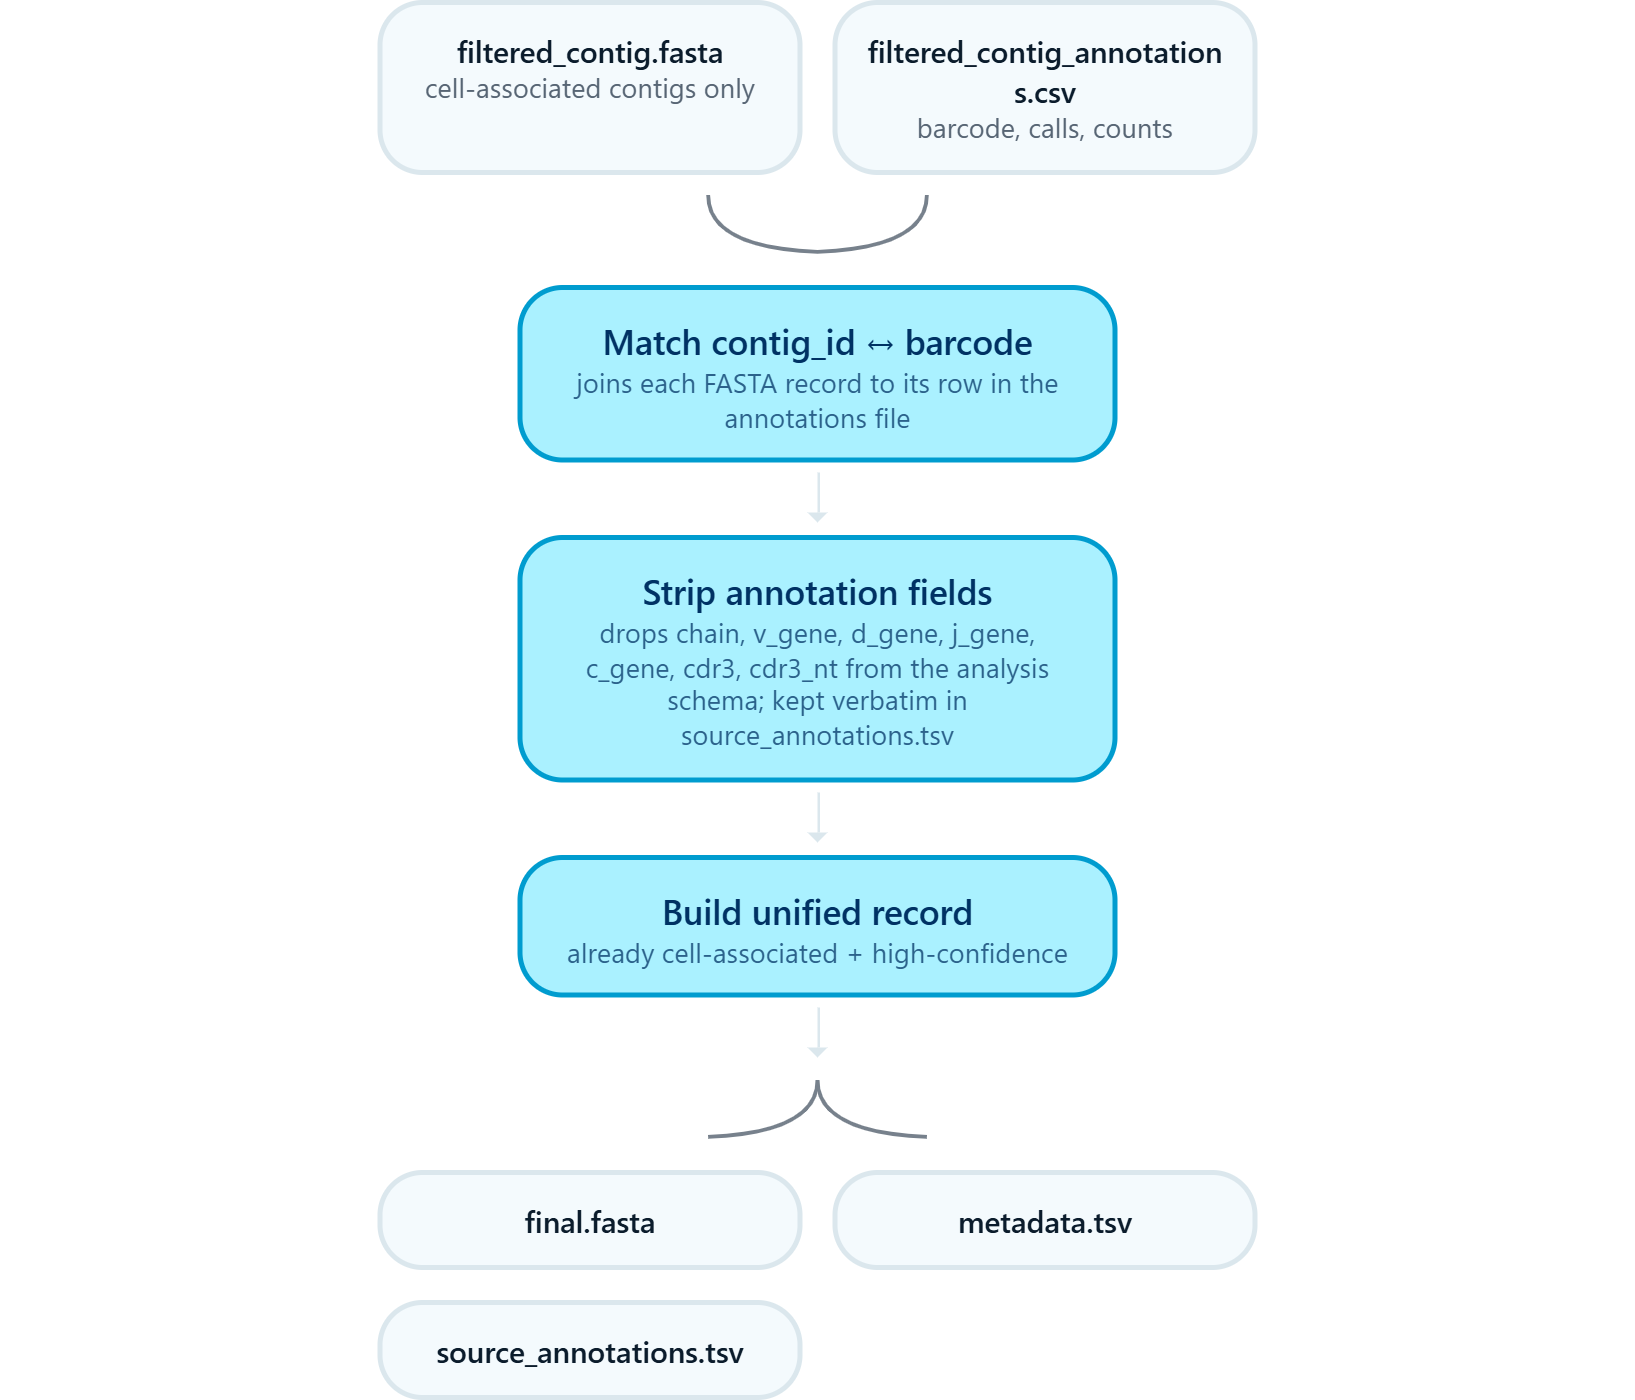
\includegraphics[width=0.75\textwidth,height=16cm,keepaspectratio]{supp_fig_S1_single_cell_workflow.png}
\caption{Representative AIRRPrep single-cell workflow visualization for a
Cell Ranger V(D)J filtered contigs input. The application displays the
processing route associated with the selected single-cell input and allows the
workflow graphic to be exported as a PNG; this figure is that export. The
annotation fields the \emph{Strip annotation fields} step removes from the
normalized record are not discarded: they are kept unchanged in
\texttt{source\_annotations.tsv}, keyed on the same \texttt{sequence\_id} as
\texttt{final.fasta} and \texttt{metadata.tsv}. The run therefore writes three
record-level outputs --- \texttt{final.fasta}, \texttt{metadata.tsv} and
\texttt{source\_annotations.tsv} --- plus the run-level
\texttt{provenance.json}, which the diagram does not show because it is written
once for the run rather than per record (Supplementary Table~S1).}

\end{figure}

\clearpage
\section*{Supplementary Figure S2. Visualization of a custom paired-read bulk workflow}
\begin{figure}[h!]
\centering
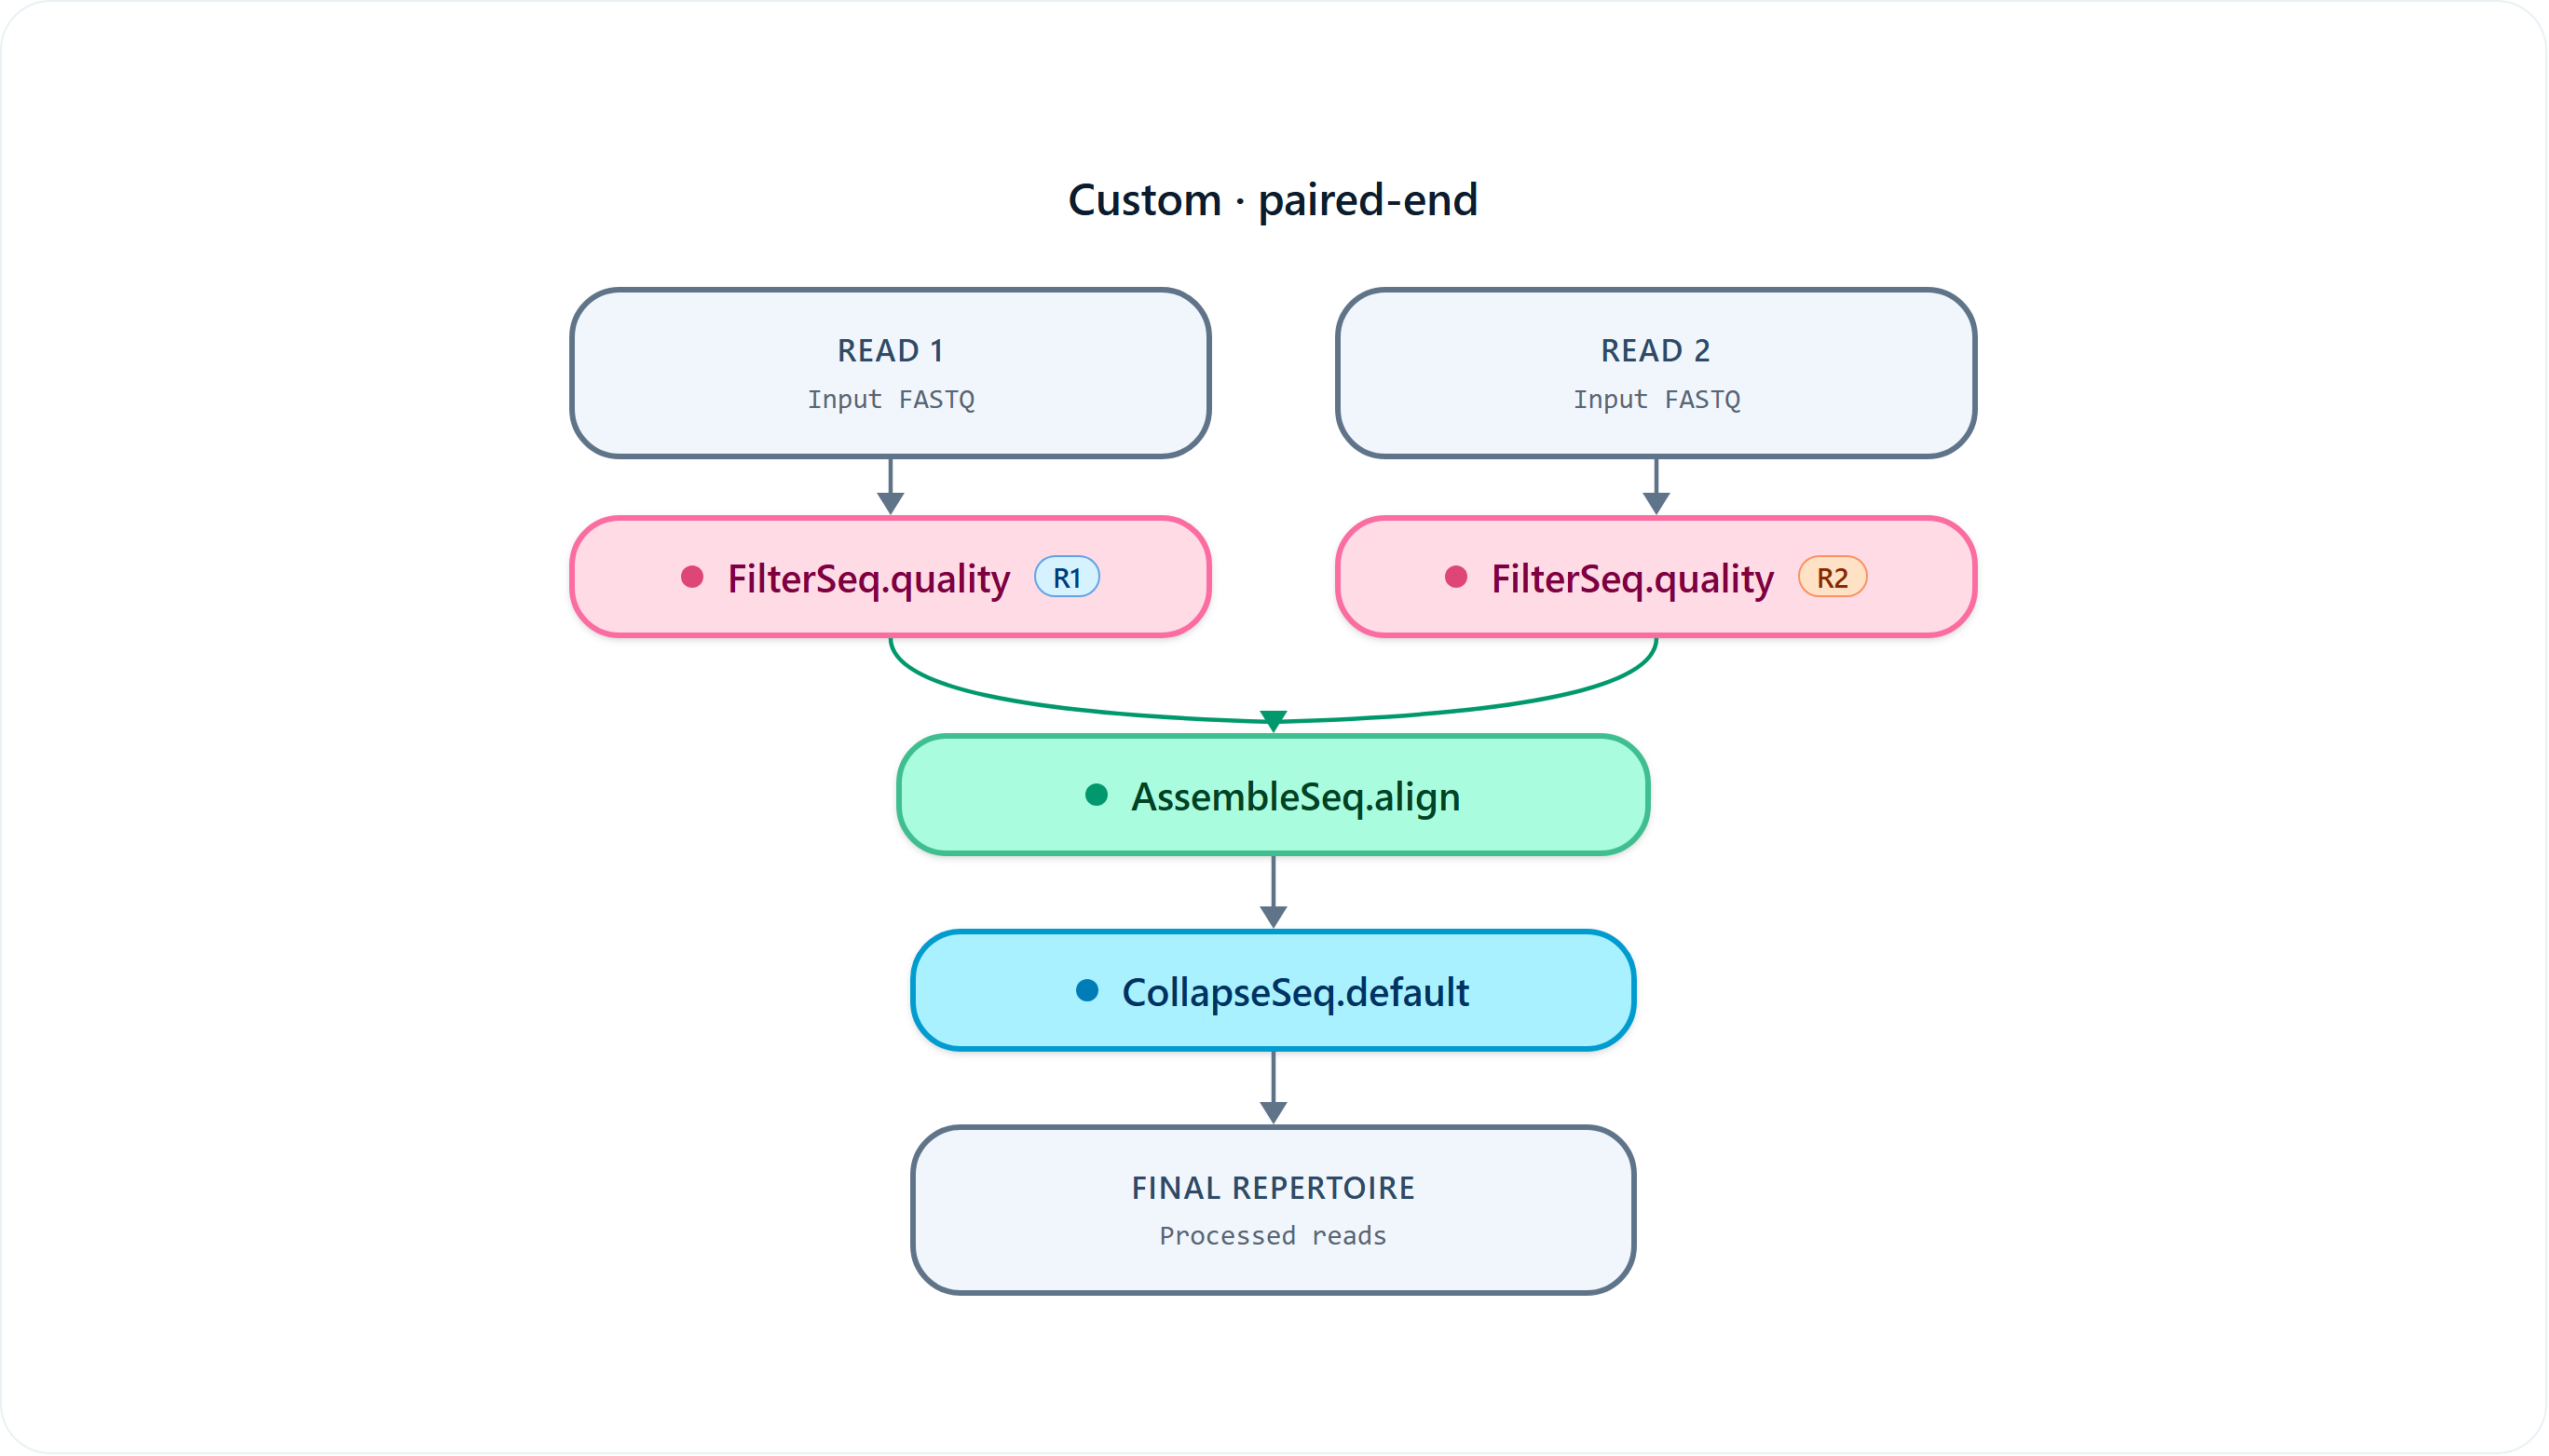
\includegraphics[width=0.75\textwidth,height=16cm,keepaspectratio]{supp_fig_S2_paired_read_workflow.png}
\caption{Representative AIRRPrep paired-read bulk workflow visualization. Read 1 (R1) and Read 2 (R2) are shown through the operations applied to each read stream and, where applicable, their transition to a merged sequence stream after assembly. The workflow graphic can be exported from AIRRPrep as a PNG.}
\end{figure}

\clearpage
\section*{Supplementary Figure S3. Stepwise read-retention visualization example}
\begin{figure}[h!]
\centering
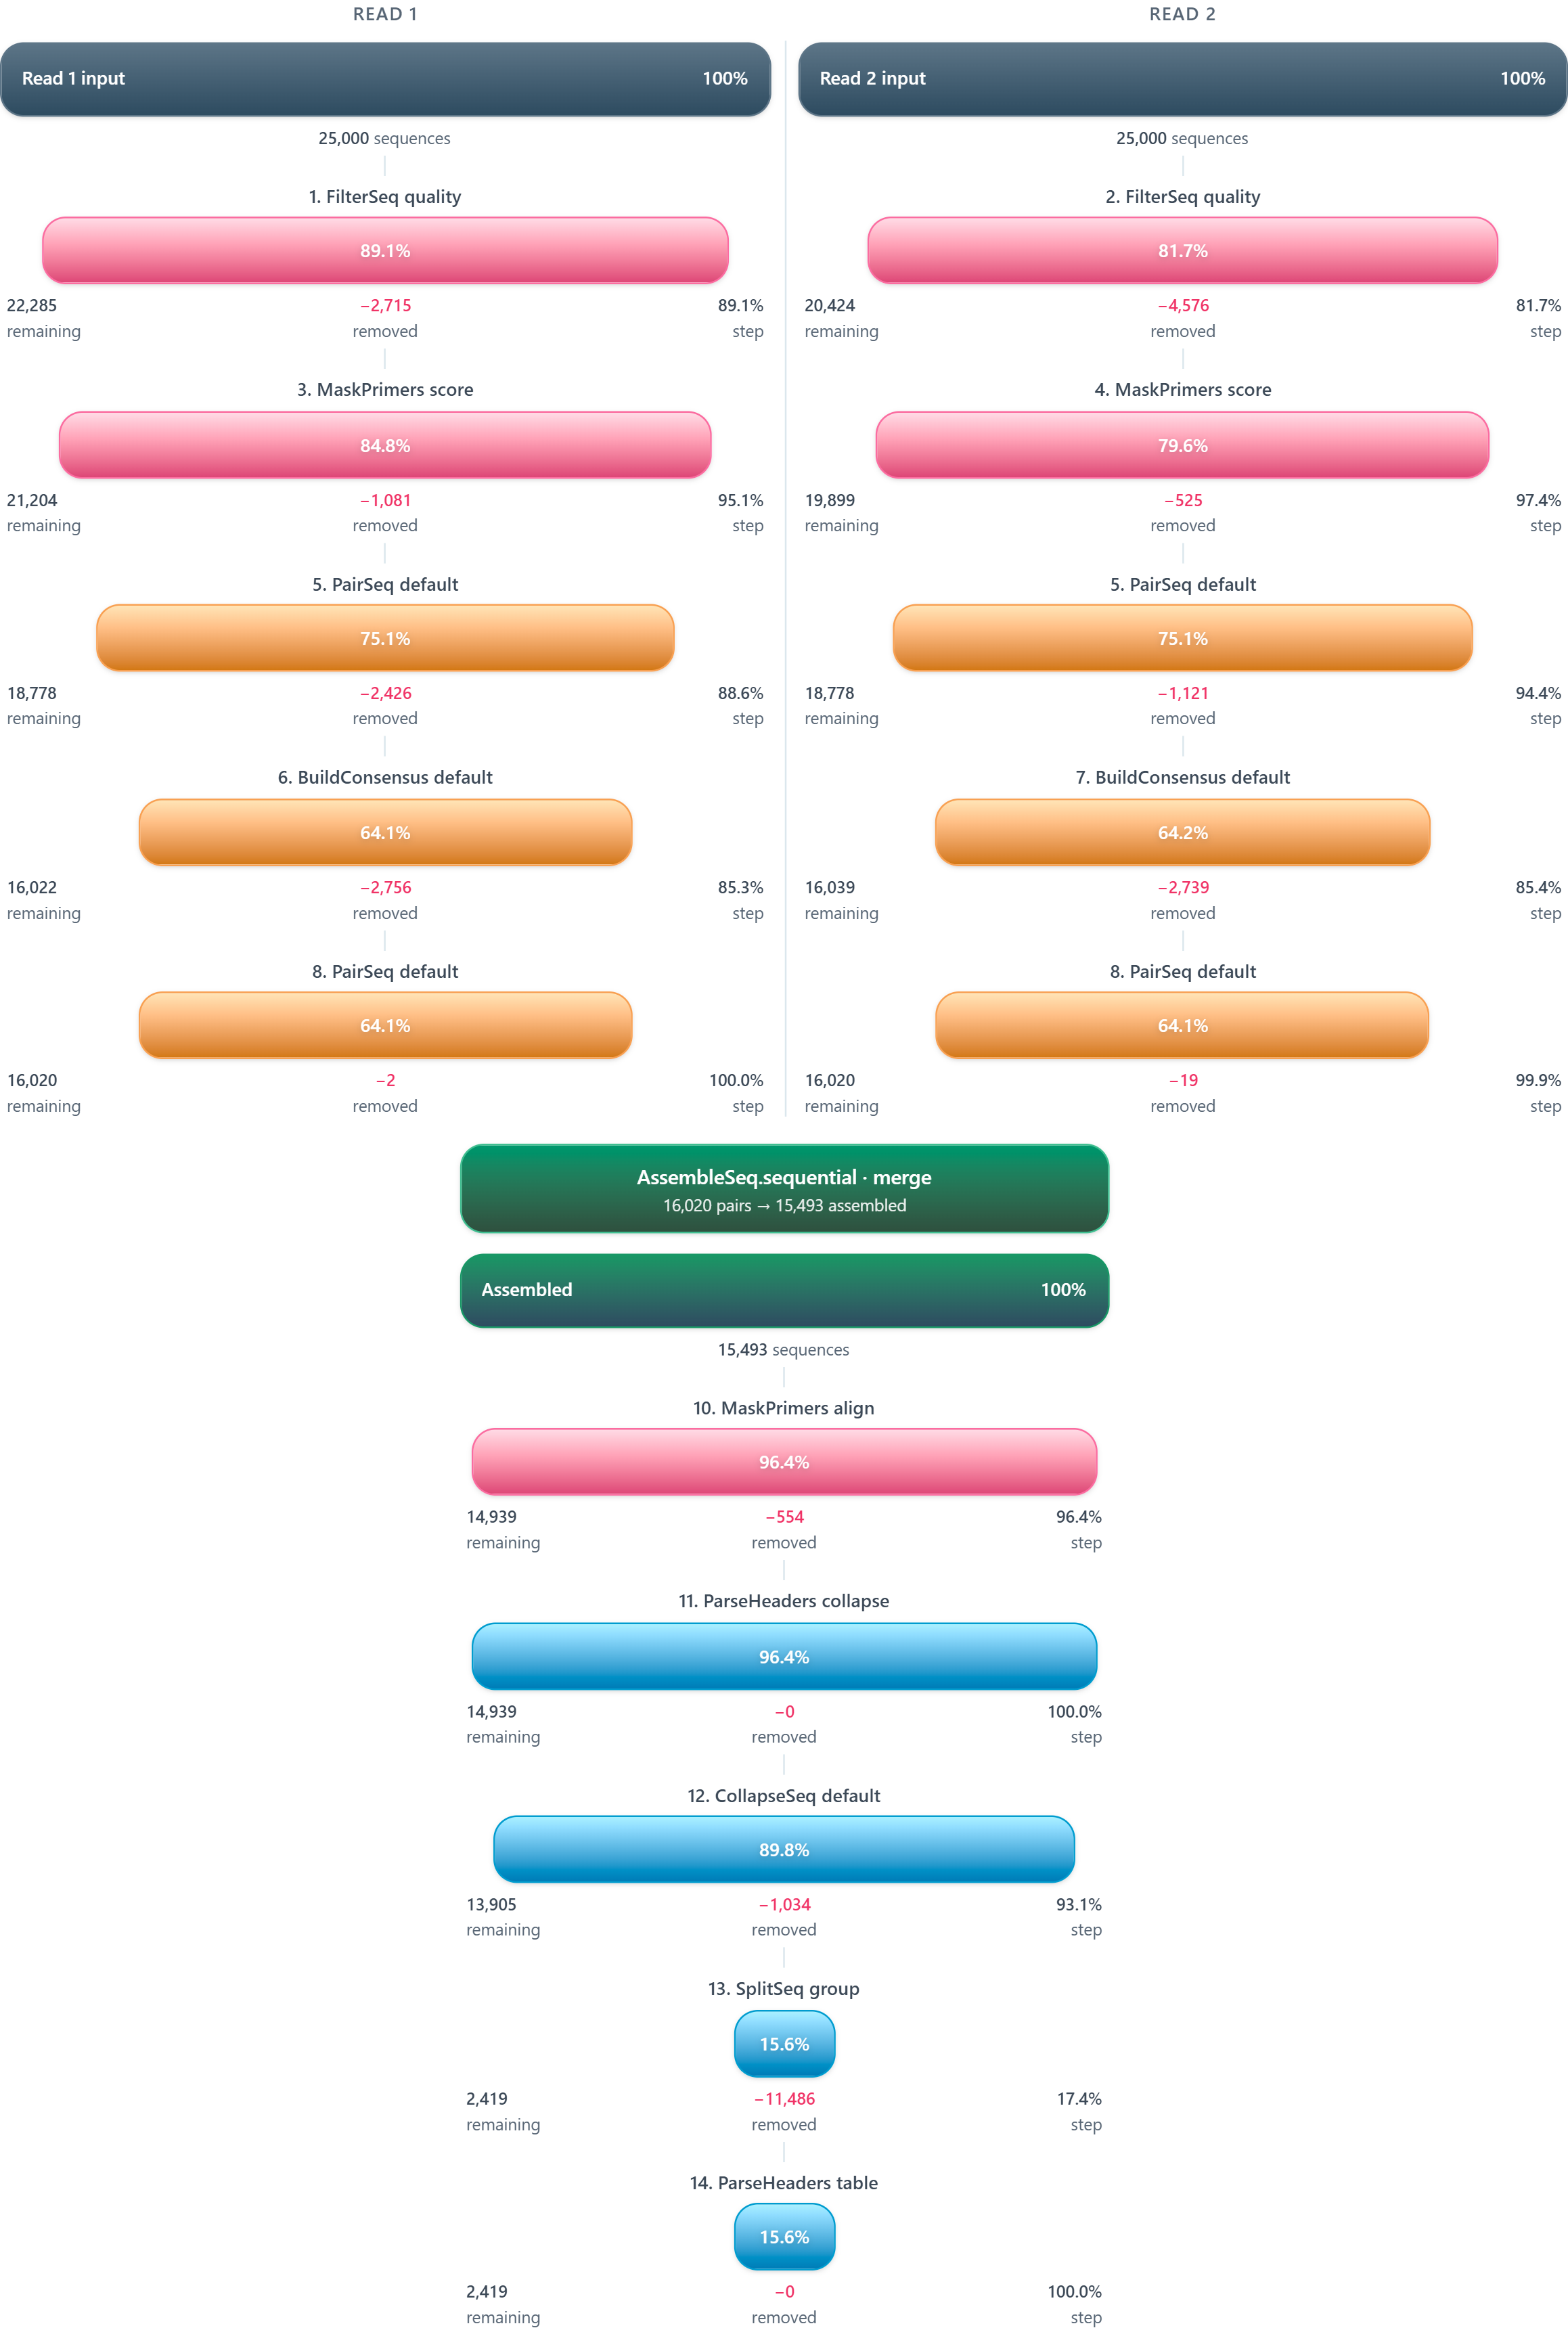
\includegraphics[width=0.75\textwidth,height=16cm,keepaspectratio]{supp_fig_S3_read_retention.png}
\caption{AIRRPrep read-retention visualization for the UMI-barcoded 5$'$ RACE MiSeq 325+275 workflow of Supplementary Table~S3 (SRR4026043, first 25,000 read pairs). Each box names its operation and shows the records entering and retained; R1 and R2 are counted separately until assembly, after which the merged stream is followed. The visualization can be exported as a PNG.}

\end{figure}

\clearpage
\section*{Supplementary Figure S4. Bulk read-stream behaviour and output rules}
\begin{figure}[h!]
\centering
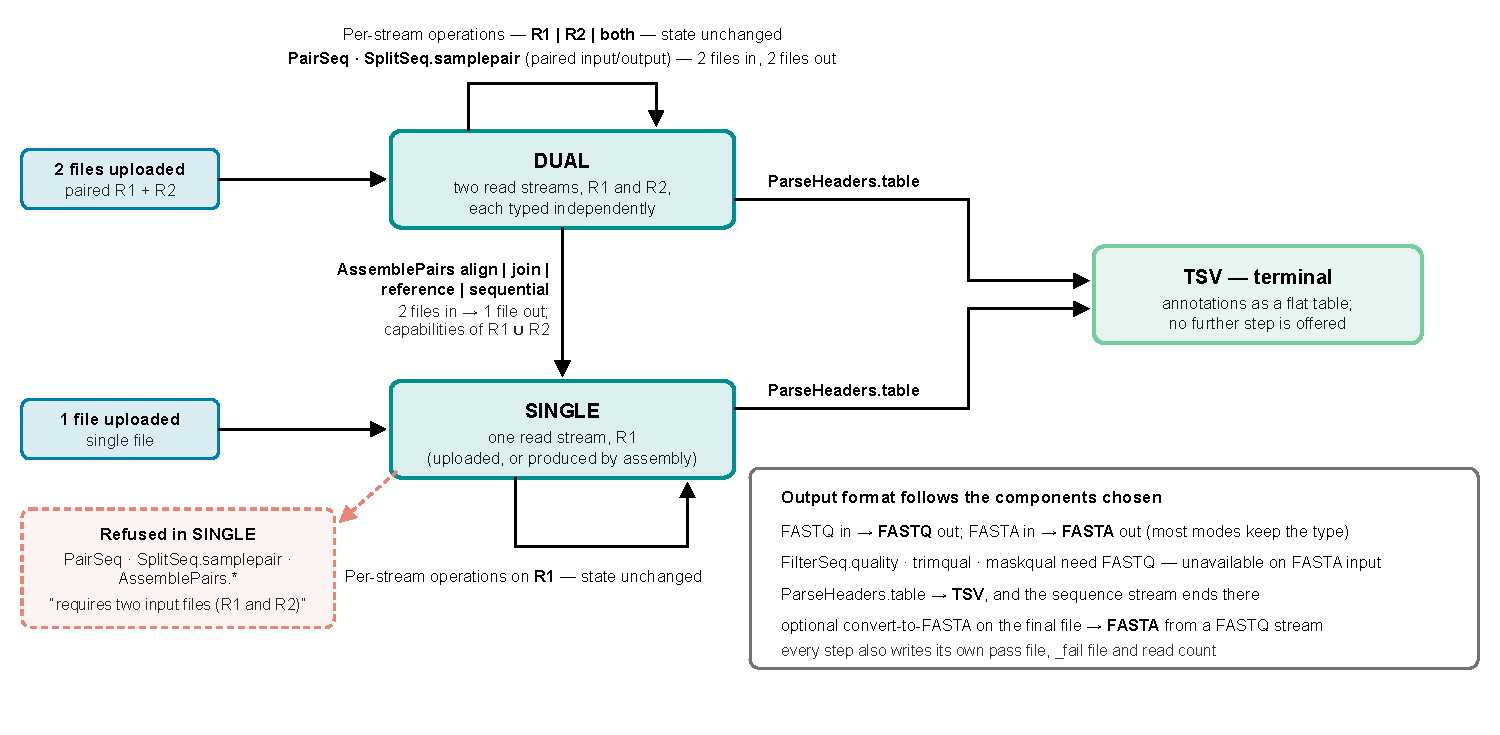
\includegraphics[width=0.98\textwidth]{figure2_bulk_read_streams.pdf}
\caption{Read-stream behaviour of bulk operations. An operation may act on
the Read 1 (R1) or Read 2 (R2) stream independently, require both streams and
keep them separate (for example \texttt{PairSeq.py}), or merge the two streams
into a single sequence stream (\texttt{AssemblePairs.py}). Read streams are
called R1 and R2 throughout this work, never ``lane'': a sequencing flow-cell
lane is a different thing, and the word is used in this supplement only where
a physical lane is meant (lane L001 in Supplementary Table~S7). The four
assembly operations, written \texttt{AssemblePairs.py align}, \texttt{join},
\texttt{reference} and \texttt{sequential} in this supplement and in every
table, are the components the interface labels \texttt{AssembleSeq.align},
\texttt{AssembleSeq.join}, \texttt{AssembleSeq.reference} and
\texttt{AssembleSeq.sequential}; that family is the only name that differs
between the interface and pRESTO (Supplementary Table~S2).}
\end{figure}




\clearpage
\section*{Supplementary Table S1. Input and output by data category}
\begin{center}
\begin{tabular}{p{0.20\textwidth}p{0.45\textwidth}p{0.25\textwidth}}
\toprule
Data category & Input & Output \\
\midrule
Bulk AIRR-seq & One sequence file, or matched R1 and R2 files of a paired-end run; FASTA or FASTQ, both files in the same format & FASTA, FASTQ or TSV \\
Single-cell AIRR & One of the seven input specifications below & \texttt{final.fasta}, \texttt{metadata.tsv}, \texttt{source\_annotations.tsv}, \texttt{provenance.json} \\
\bottomrule
\end{tabular}
\end{center}

\begin{center}
\small
\begin{tabular}{p{0.05\textwidth}p{0.25\textwidth}p{0.62\textwidth}}
\toprule
\textbf{ID} & \textbf{Specification} & \textbf{Required files} \\
\midrule
1 & Cell Ranger, all contigs & \texttt{all\_contig.fasta} + \texttt{all\_contig\_annotations.csv} \\
2 & Cell Ranger, filtered contigs & \texttt{filtered\_contig.fasta} + \texttt{filtered\_contig\_annotations.csv} \\
3 & Cell Ranger AIRR table & \texttt{airr\_rearrangement.tsv} \\
4 & TRUST4 output & \texttt{*\_annot.fa} + \texttt{*\_barcode\_report.tsv}, from one TRUST4 run in barcode mode \\
5 & Raw 10x FASTQ & R1 FASTQ (cell barcode + UMI) + R2 FASTQ (cDNA); assembled with TRUST4 \\
6 & 10x BAM & genome-aligned BAM with CB/UB tags (e.g.\ \texttt{possorted\_genome\_bam.bam}); assembled with TRUST4 \\
7 & Generic FASTA & receptor FASTA + barcode mapping file (\texttt{sequence\_id}, \texttt{cell\_id}, \texttt{umi\_count}, \texttt{read\_count}) or a header regular expression \\
\bottomrule
\end{tabular}
\end{center}

{\small\textit{Supplementary Table S1.} Supported input and output file types
for bulk and single-cell AIRR-seq data, and the seven single-cell input
specifications. The two Cell Ranger contig sets are counted as separate
specifications because they are different files with different content. When
an uploaded file set matches a specification only in part, the application
names the companion files needed to complete it. Single-cell input is not
processed through a user-composed chain, because upstream software may already
have reconstructed contigs; each specification has one adapter. The
single-cell output is AIRRPrep's internal normalized representation, not an
AIRR Rearrangement record, with eight fields: \texttt{sequence\_id} (the source
record's own identifier, unchanged), \texttt{sequence}, \texttt{cell\_id},
\texttt{umi\_count}, \texttt{read\_count}, \texttt{is\_cell},
\texttt{high\_confidence} and \texttt{productive}. A value the source does not
carry is left empty rather than inferred, and \texttt{productive} is filled only
when the user opts in, for Cell Ranger input.

Upstream V(D)J calls, junctions and CDR3 annotations are excluded from that
normalized record so that every sequence is re-annotated with one reference
and one procedure. Excluding them from the analysis schema does not destroy
them: every field the uploaded file carried for a record --- the contig
annotations CSV or AIRR TSV row, the barcode mapping file row, the FASTA
header, TRUST4's \texttt{annot.fa} header and its barcode-report and
\texttt{barcode\_airr} rows --- is written verbatim to
\texttt{source\_annotations.tsv}, one row per output record, keyed on the same
\texttt{sequence\_id}. An inner join on that column is total and
collision-free, so any omitted annotation can be restored without the original
upload. \texttt{provenance.json} records the name, size and SHA-256 checksum of
every input and of every output including the sidecar, which files the sidecar
was read from, the adapter options, software versions and parse counts; a
checksum of the source file therefore verifies the identity of that file,
while the sidecar is what preserves its annotation content. The join is
covered by an automated test
(\texttt{presto-backend/tests/test\_source\_annotations.py}), which asserts
that every normalized record has exactly one sidecar row, that no identifier
is duplicated or lost on either side, and that the fields the normalized
output omits are present in the sidecar with the values the source gave.\par}

\textit{Note:} In the hosted deployment an uploaded file may be up to 200~MB
and one session may hold up to 2~GB of uploads; uploaded files are retained for
ten days and can be reused across runs within that window, and a job recovered
with a tracking code remains available for seven days. All four limits are
deployment settings (Supplementary Note~S2).


\clearpage
\section*{Supplementary Table S2. Bulk pRESTO operations exposed by AIRRPrep}

AIRRPrep exposes 47 operations drawn from 13 pRESTO tools. Each operation
listed below has exactly one archived test case, run within AIRRPrep and
natively on the same input and the two outputs compared; those 47 cases are
the denominator of every count reported in this section, and the scope of the
comparison is stated in the subsection after the table. A separate,
additional test covers the three \texttt{ClusterSets} operations with the
proprietary USEARCH, which is not part of the 47 and is reported on its own at
the end of this section.

\begin{longtable}{p{0.21\textwidth}p{0.42\textwidth}p{0.29\textwidth}}
\toprule
Tool & Description & Operations exposed \\
\midrule
\endhead
\texttt{AlignSets.py} & Multiple-aligns sets of sequences sharing the same annotation & \texttt{muscle}, \texttt{offset}, \texttt{table} (3) \\
\texttt{AssemblePairs.py} & Assembles paired-end reads into a single sequence & \texttt{align}, \texttt{join}, \texttt{reference}, \texttt{sequential} (4) \\
\texttt{BuildConsensus.py} & Builds a consensus sequence for each UMI/barcode group & single operation (1) \\
\texttt{ClusterSets.py} & Clusters read groups & \texttt{all}, \texttt{barcode}, \texttt{set} (3)\textsuperscript{a} \\
\texttt{CollapseSeq.py} & Removes duplicate sequences while recording duplicate counts & single operation (1) \\
\texttt{ConvertHeaders.py} & Converts sequence headers into pRESTO format & \texttt{454}, \texttt{genbank}, \texttt{generic}, \texttt{illumina}, \texttt{imgt}, \texttt{migec}, \texttt{sra} (7) \\
\texttt{EstimateError.py} & Estimates error rates for UMI data & \texttt{barcode}, \texttt{set} (2) \\
\texttt{FilterSeq.py} & Removes or modifies low-quality reads & \texttt{length}, \texttt{quality}, \texttt{missing}, \texttt{repeats}, \texttt{trimqual}, \texttt{maskqual} (6) \\
\texttt{MaskPrimers.py} & Identifies and removes or masks primers while annotating the match & \texttt{align}, \texttt{extract}, \texttt{score} (3) \\
\texttt{PairSeq.py} & Synchronizes paired R1/R2 files and copies annotations between mates & single operation (1) \\
\texttt{ParseHeaders.py} & Manipulates sequence annotations and can export them as a table & \texttt{add}, \texttt{collapse}, \texttt{copy}, \texttt{delete}, \texttt{expand}, \texttt{merge}, \texttt{rename}, \texttt{table} (8) \\
\texttt{SplitSeq.py} & Splits, groups, sorts, samples and selects sequence files & \texttt{count}, \texttt{group}, \texttt{sample}, \texttt{samplepair}, \texttt{select}, \texttt{sort} (6) \\
\texttt{UnifyHeaders.py} & Unifies annotation fields by a grouping scheme & \texttt{consensus}, \texttt{delete} (2) \\
\midrule
\textbf{13 tools} & & \textbf{47 operations} \\
\bottomrule
\end{longtable}

\textsuperscript{a}~Counted once each in the 47 cases, with VSEARCH~2.31.0 as
the clustering backend --- the open tool the container image carries and the
one a deployment uses unless it is changed. AIRRPrep issues the clustering
command itself rather than through the pRESTO helper, whose USEARCH command
line the tested USEARCH build rejects; the clustering parameters exposed to
the user are unchanged. The USEARCH backend is covered by the separate test
described at the end of this section.

{\small\textit{Supplementary Table S2.} The 47 bulk-processing operations
exposed by AIRRPrep across the 13 underlying pRESTO tools that provide them,
with a short description of each tool's function. Each operation has exactly
one archived test case comparing it with the equivalent native pRESTO command,
and those 47 cases are the denominator used throughout this section. The
per-case record is released with the source code as
\texttt{paper/test/component\_matrix/component\_matrix.tsv} and
\texttt{component\_matrix.json}, one row per case with the operation, the
denominator it belongs to, the host it ran on, the input file, the parameters,
the native command, the AIRRPrep call, the comparator, the status and the
SHA-256 of each side's output set; the separate USEARCH test is released
beside it as
\texttt{usearch\_clustersets.tsv} and \texttt{usearch\_clustersets.json}. The
results are summarized below.\par}

\textit{Note:} This supplement uses pRESTO's program names throughout. The
interface labels one family differently: \texttt{AssembleSeq.align},
\texttt{.join}, \texttt{.reference} and \texttt{.sequential} in the interface,
in saved workflows and in job logs are \texttt{AssemblePairs.py align},
\texttt{join}, \texttt{reference} and \texttt{sequential}; every other
component is named \texttt{Tool.subcommand} after its pRESTO program. \texttt{ParseLog.py}, which parses pRESTO
log files after a run, is not exposed as a pipeline component, because AIRRPrep
reports the per-step record counts directly (Supplementary Figure~S3).

\subsection*{Validation of AIRRPrep on pRESTO Components}

\textbf{Scope of the component comparison.} Each of the 47 operations in
Supplementary Table~S2 has one archived test case, run through AIRRPrep's own
step executor (\texttt{run\_pipeline\_step}, the function a job calls for each
step, with the parameters the web interface sends) and as the equivalent native
pRESTO command on the same input, with the two outputs compared. The inputs are
the first 8,000 read pairs of SRR1383456 and intermediates derived from them
with native pRESTO, so no AIRRPrep output is ever the input of a test; the
\texttt{ConvertHeaders} cases use 500 of those reads with headers rewritten into
each vendor format, and reference-guided assembly uses 300 read pairs because it
calls BLAST once per pair. The case list, parameters, commands and per-case
results are archived with the source code
(\texttt{paper/test/component\_matrix/}), as is the harness that produces them.

Outputs are compared by content, not by file layout. Sequence outputs are
compared as record sets --- identifier, sequence, quality string and the
annotation field/value set --- with pass and failed records compared separately
(for read-pair assembly the two sides group failed records differently, pRESTO
writing one file per input and AIRRPrep one file per step, so those records are
compared as one set per side);
an operation that fans out into several files must match one native file per
AIRRPrep file; table outputs are compared as sets of rows keyed by column name;
random sampling, which pRESTO does not seed, is checked for equal size, absence
of duplicates and membership of every sampled record in the input; and
clustering is checked for identical records apart from the cluster label
together with an identical partition of records into clusters.

\textbf{Result.} Of the 47 cases, 46 are comparable and all 46 produced
identical output on both sides, over 123,016 compared sequence records in the
record-set cases plus the fan-out, table, sampling and clustering cases. The
47th, \texttt{ConvertHeaders.py migec}, is \emph{not comparable}: native pRESTO
refuses its own documented input, so there is no native output to compare
against, and AIRRPrep's run of it is reported as a native failure rather than
as agreement (below). Every case therefore carries exactly one of two
statuses, \emph{identical} or \emph{not comparable (native pRESTO failed)}, and
their counts are 46 and 1.

Five of the 47 cases were run in a Linux container rather than on the benchmark
host, because they cannot run on Windows at all: pRESTO passes those external
tools a temporary file while Python still holds it open, which Windows does not
permit, so \emph{both} implementations fail and nothing can be compared.
This affects the three \texttt{ClusterSets} operations, where VSEARCH reports
that it cannot open the \texttt{uc} file, and the two reference-guided assembly
operations, where \texttt{makeblastdb} writes no database and every read pair is
consequently reported as unassembled. The container is built from the same
pRESTO version and the official VSEARCH and BLAST+ releases, pinned by checksum
(Supplementary Table~S10). Which host ran each case is recorded per case in the
released report.

This per-operation matrix and the whole-workflow comparison of Supplementary
Tables~S3--S5 answer different questions. The workflows show that 11 operations
behave identically in composition, over 25,000 read pairs and with each step's
output feeding the next; the matrix shows that each of the 46 comparable
operations behaves identically in isolation, including those no predefined
workflow uses. No claim of identical behaviour is made for
\texttt{ConvertHeaders.py migec}, which has no native counterpart to be
identical to.

\textbf{The one case that could not be compared.} \texttt{ConvertHeaders.py
migec} is the 47th case, and native pRESTO refuses its own documented input.
MIGEC writes every record as \texttt{@MIG UMI:\textit{barcode}:\textit{count}},
so the leading token is \texttt{MIG} in every record; pRESTO counts the records of an
input file by building a Biopython index keyed on that token, which raises
\texttt{Duplicate key 'MIG'} and ends the run before any header is converted.
Any MIGEC file with more than one record is affected. AIRRPrep streams the file
instead of indexing it and converts it with pRESTO's own
\texttt{convertMIGECHeader} function, so the conversion is pRESTO's; what
differs is only the file handling around it. Because native pRESTO writes no
output, there is nothing to compare the 500 converted records against, and the
case is reported as \emph{not comparable}, not as agreement.

\subsection*{Separate test: \texttt{ClusterSets} with USEARCH}

The three \texttt{ClusterSets} cases of the matrix above use VSEARCH. USEARCH
is tested separately, for two reasons: counting the same three operations twice
would make the denominator ambiguous, and USEARCH is proprietary, so a reader
cannot repeat that test without a licence of their own. It is therefore
reported here, on its own, and is archived separately as
\texttt{paper/test/component\_matrix/usearch\_clustersets.tsv} and
\texttt{.json}, produced by \texttt{run\_usearch\_clustersets.py}.

Native pRESTO cannot run \texttt{ClusterSets.py} with USEARCH at all, because
of the command line pRESTO constructs rather than any parameter chosen by the
user. pRESTO builds its USEARCH invocation with the \texttt{-minwordmatches}
option, which USEARCH v7.0.1090 -- the build tested here, and the series pRESTO
documents for this step -- does not recognise; USEARCH exits with
\texttt{Invalid command line}, \texttt{Unknown option minwordmatches}, and
pRESTO reports the step as failed. Because the option is part of the command
pRESTO constructs, the failure occurs for any input and cannot be avoided
through the parameters the tool exposes. All three operations
(\texttt{all}, \texttt{barcode}, \texttt{set}) fail identically.

AIRRPrep therefore issues the clustering command itself instead of delegating
to the pRESTO helper. The USEARCH invocation omits the unsupported option; the
VSEARCH invocation passes it in VSEARCH's long-option form
(\texttt{-{}-minwordmatches}); and the thread count is omitted from the command
when it has not been configured, rather than being interpolated as the literal
string \texttt{None}. With that invocation USEARCH accepts the command line and
starts, for all three operations.

The comparison cannot be carried through to an output check on the benchmark
host, for the same reason the three VSEARCH cases of the matrix are run in the
Linux container: pRESTO hands the external tool a temporary file that Python
still holds open, and on Windows USEARCH then reports
\texttt{Cannot open \ldots errno=13 Permission denied}. Doing for USEARCH what
was done for VSEARCH would require a licensed Linux USEARCH binary inside the
test container, which cannot be redistributed with the test suite. What is
established here is therefore exactly this: the command line native pRESTO
generates is rejected by USEARCH, and the one AIRRPrep generates is not. The
clustering parameters exposed to the user -- identity threshold, length ratio,
sequence window and choice of clustering tool -- are unchanged either way.

USEARCH is proprietary and is not distributed with AIRRPrep or its container
image; a deployment that holds a USEARCH licence supplies its own binary
through the \texttt{USEARCH\_BIN} setting, and selecting USEARCH without one
fails with a message naming the licence requirement rather than a missing
executable. No default selects it: clustering defaults to VSEARCH and
reference-guided assembly to BLAST+, both of which the image carries. That the
released tree and image contain no USEARCH binary, that nothing in the build
installs one, and that no predefined workflow needs one, are asserted by
automated tests
(\texttt{presto-backend/tests/test\_no\_proprietary\_binaries.py}). The USEARCH
and VSEARCH versions used are listed in Supplementary Table~S10.

\clearpage
\section*{Supplementary Note S1. Declarative Workflow Validation and Interactive Constraint Enforcement}

Workflow validation in AIRRPrep is implemented within the framework itself and
is not inherited from the underlying toolkits. pRESTO validates the arguments
of an individual command at the time that command is executed, but it does not
establish whether a sequence of commands is coherent with respect to the files
actually supplied. In a command-line setting an incompatibility of this kind is
therefore discovered only when the offending step runs, after the preceding
steps have already been executed, and in some cases only in the form of a
silently empty output file.

Every operation exposed by AIRRPrep declares a contract: the file types it
accepts, the annotation capabilities it requires and the capabilities it
produces, the companion files it needs (for example a primer FASTA), and
whether it acts on one read stream, requires both the Read~1 (R1) and Read~2
(R2) streams, or merges them into one. Capabilities are tracked separately for
the R1 and R2 streams. Before a job is dispatched, the selected workflow is
replayed symbolically over the uploaded files: the file type and the capability
state of each read stream are updated after every operation, and execution is
refused at the first step whose contract is not satisfied. The resulting error
identifies the failing step, the affected read stream and the specific unmet
requirement. Representative constraints enforced by this mechanism include
consensus building before barcode annotation has been created, paired
operations on single-file input, quality-based filtering on FASTA input, which
carries no quality scores, and primer masking without the required primer
FASTA.

The same contracts are evaluated interactively while a custom workflow is being
constructed. The set of selectable components is recomputed after every change
to the uploaded input set or to the pipeline, so that components whose input
types or required capabilities are not satisfied in the current state are
disabled, whereas components become available as soon as their prerequisites
are produced by an earlier step or supplied by an additional input file.
Selecting an operation immediately updates which downstream operations are
offered, uploading a different input type or a companion file re-enables the
operations that depend on it, and a disabled component reports the requirement
it is missing rather than being unavailable without explanation. Because only
operations that are valid for the current data can be selected, assembling a
valid pipeline does not require prior knowledge of the correct ordering of
preprocessing steps. The same operation contracts are also used to generate the
in-application documentation, so the documented requirements and the enforced
requirements cannot diverge, and each predefined workflow is shown with a
schematic of the library design it targets.

The same mechanism is applied a level deeper, to individual parameters rather
than whole operations. Several operations take an annotation field name as a
parameter -- the field an operation groups, sorts or filters by, for example,
or the annotations two paired-end reads exchange -- and which field names are
actually present depends on the specific workflow assembled so far: it begins
with the fields detected in the uploaded file's headers and changes as
operations that add, rename, merge or remove annotations are added, so it
cannot be read off the operation's contract alone. AIRRPrep tracks this
field-name set per read stream alongside the capability state described
above, and wherever a parameter names an existing or new field, offers it as
a choice drawn from that tracked set rather than requiring the name to be
typed. When
the uploaded header format has not yet been normalized to pRESTO's convention
-- before the corresponding header-conversion operation has been applied, for
instance -- the tracked set may be incomplete, and a typed value remains
available alongside it, since an unconfirmed field list must not silently
reject a name it has simply not seen yet. The same field-existence check is
applied once more, non-interactively, when the workflow is dispatched.

\textbf{Tests of the validator.} The job-launch validator is covered by an
automated test suite (\texttt{presto-backend/tests/test\_workflow\_validation.py})
that runs it on freshly written FASTQ and FASTA files without pRESTO
annotations, the state of a new upload. The three predefined workflows must be
accepted, and each of the following 14 deliberately invalid compositions must
be refused at the step at fault:
\begin{center}
\small
\begin{tabular}{p{0.28\textwidth}p{0.64\textwidth}}
\toprule
\textbf{Class} & \textbf{Invalid composition (expected: refused)} \\
\midrule
Missing annotation & consensus building on reads without a barcode; the UMI 2$\times$250 workflow without the \texttt{PairSeq.py} step that copies the barcode to R2 \\
Incorrect file type & quality filtering on FASTA; R1 FASTQ with R2 FASTA \\
Absent companion file & primer masking without a primer FASTA; reference-guided assembly without a reference \\
Invalid read-stream state & \texttt{PairSeq.py} on single-file input; \texttt{AssemblePairs.py} on single-file input; an R2 operation on single-file input \\
Impossible operation order & an R2 operation after the streams were merged; \texttt{PairSeq.py} after assembly; any operation after a split into an unbounded number of files; a field parameter naming an annotation that does not exist at that point \\
Unknown operation & a component name the server does not provide \\
\bottomrule
\end{tabular}
\end{center}
All 3 valid workflows were accepted and all 14 invalid compositions were
refused with an error naming the failing step (no false acceptance and no
false rejection on this set). The set is designed to cover each class of
constraint the contracts express, not to estimate error rates over arbitrary
user-built workflows.

\clearpage
\section*{Supplementary Note S2. Managing Data, Workflows, and Running Jobs}

\textbf{Sessions and uploaded files.} AIRRPrep requires no account. Work is
organized in a browser session, which is issued its own secret token; every
session, file and job route is authorized against that token, and only a hash
of it is stored. Uploaded files belong to the session and are retained for ten
days, so a second workflow can reuse a file that has already been uploaded
rather than transferring it again; the interface shows the remaining retention
time, so reuse is an informed choice. A session may hold up to 2~GB of uploads
with a ceiling of 200~MB per file, and both limits, like the retention window,
are deployment settings. Jobs previously run in a session remain listed with
their status, a running job can be cancelled, and the output of an individual
step -- including the \texttt{\_fail} file of a filtering step -- can be
downloaded on its own or the complete set of job outputs as a single archive.
Because the service is public, uploads are restricted by file type and size,
and requests are rate limited per client address.

\textbf{Saved and exported workflows.} A workflow assembled in the custom
builder can be saved under the session and exported as a machine-readable
definition, which can be imported again -- into another session, or by another
user -- to reproduce the same operation sequence and parameters. A finished run
can likewise be saved as a reusable workflow. Parameters that reference an
uploaded file, such as a primer FASTA, are deliberately not embedded in the
saved definition: uploads expire, and a stored reference to a file that no
longer exists would fail at launch with an identifier the user cannot
interpret. Such parameters are stripped on save and recorded instead as
required inputs, each named together with the step that consumes it, so
re-running asks for the primer FASTA again explicitly and by name. When the
parameter named one of the session's own uploads at the time of saving, the
entry also records that file's original name, size and SHA-256 checksum, and
the definition records the AIRRPrep, pRESTO and Python versions under which it
was saved and exported (an image digest as well, when the deployment sets it).
The exported definition is therefore a reusable workflow definition that
identifies every companion file by content; with the accessions of the
sequencing inputs and the digest of the container image, it identifies the
preprocessing that was applied.

\textbf{Long-running jobs, notification and recovery.} Before a job starts,
AIRRPrep estimates its runtime from the size of the input and from the
throughput of the operations the workflow contains, since throughput differs by
more than an order of magnitude between, for example, a per-read quality
predicate and a local alignment against every primer. Runs the estimator
considers long may be started only from a session that has verified an email
address; the estimate is a sizing heuristic and errs towards over-estimation,
and the requirement is enforced by the backend rather than by the interface.
Any session with a verified address is notified when its jobs start and when
they finish or fail, whether or not the run was long.

The start notification carries a six-digit tracking code that restores the run
on the page it was launched from, from any browser or machine, for seven days.
A six-digit code is short enough to quote or write down, and correspondingly
too small a space to serve as a credential on its own, so recovery requires the
code together with the address it was issued to. For the same reason the link
in the email pre-fills only the code, never the address.

\textbf{Handling of email addresses and recovery controls.} The address a user
verifies is kept in plain text on the session record and on the records of
jobs started from that session, because it is needed to deliver the start and
completion notifications; those records expire with the session and job
retention periods. Mail is sent by the backend over SMTP to the operator's
configured mail server. The tracking record that a recovery looks up does not
contain the address: it stores an HMAC-SHA256 of the normalized address, keyed
with a server-side secret held in the deployment environment rather than in the
data store, so a copy of the data store alone does not allow addresses to be
recovered by hashing candidate addresses. The same code and a different address
give the same failure as an unknown code, so the route does not reveal which
codes exist. Verification codes expire after 15 minutes, are stored only as a
salted hash, are invalidated after five wrong attempts, and cannot be resent to
a session within 60 seconds. The recovery route requires a solved CAPTCHA before
any lookup and is limited to ten requests per minute per client address (five
per minute for sending a verification code); tracking codes expire seven days
after their last use. All of these values are deployment settings.

Every statement in this paragraph is covered by an automated test
(\texttt{presto-backend/tests/test\_security\_controls.py}), which runs against
an in-memory store with an injectable clock, so expiry and cooldowns are
checked without a server and without waiting: code expiry and that a wrong
guess does not extend it, the attempt limit and that it burns the code, the
resend cooldown, storage as a salted hash only, address normalisation and the
refusal of malformed addresses, the keyed HMAC on the tracking record, the
identical answer for a wrong code and a wrong address, the absence of the
address from the recovery link, the rate limits, and the consumption of a
CAPTCHA on first use whether the answer was right or wrong. What the operator
must supply rather than the code enforce --- the HMAC secret, TLS in front of
the service, the SMTP configuration, the retention policy of the plain-text
addresses on session and job records --- is set out in \texttt{SECURITY.md} in
the repository.

\clearpage
\section*{Supplementary Table S3. AIRRPrep and CLI-pRESTO: Comparison of Processing Results for the UMI-barcoded Illumina MiSeq 325+275 paired-end 5$'$ RACE BCR mRNA validation workflow}
The predefined UMI-barcoded 5$'$ RACE MiSeq 325+275 workflow was run on the
first 25,000 read pairs of SRR4026043. Step parameters are given in
Supplementary Table~S9.

\begin{center}
\small
\begin{tabular}{clllll}
\toprule
\textbf{Step} & \textbf{Operation} & \textbf{Stream} & \textbf{Input} & \textbf{AIRRPrep} & \textbf{CLI-pRESTO} \\
\midrule
1--2 & FilterSeq.quality & R1 / R2 & 25,000 / 25,000 & 22,285 / 20,424 & 22,285 / 20,424 \\
3--4 & MaskPrimers.score & R1 / R2 & 22,285 / 20,424 & 21,204 / 19,899 & 21,204 / 19,899 \\
5 & PairSeq & paired & 21,204 + 19,899 & 18,778 pairs & 18,778 pairs \\
6--7 & BuildConsensus & R1 / R2 & 18,778 & 16,022 / 16,039 & 16,022 / 16,039 \\
8 & PairSeq & paired & 16,022 + 16,039 & 16,020 pairs & 16,020 pairs \\
9 & AssemblePairs.sequential & merged & 16,020 & 15,493 & 15,493 \\
10 & MaskPrimers.align & merged & 15,493 & 14,939 & 14,939 \\
11 & ParseHeaders.collapse & merged & 14,939 & 14,939 & 14,939 \\
12 & CollapseSeq & merged & 14,939 & 13,905 & 13,905 \\
13 & SplitSeq.group & merged & 13,905 & 2,419 & 2,419 \\
\bottomrule
\end{tabular}
\end{center}

{\small\textit{Supplementary Table S3.} Number of records retained after each
processing step of the UMI-barcoded 5$'$ RACE MiSeq 325+275 workflow
(SRR4026043, first 25,000 read pairs), for AIRRPrep and the equivalent
command-line pRESTO implementation (records retained). At every step the two
implementations wrote the same records: every sequence identifier was present
on both sides with an identical nucleotide sequence, quality string and
annotation set (compared as a multiset of field--value pairs, so that a
repeated field counts as a difference while a reordering does not), with no
missing, additional or altered record; PairSeq steps were compared mate by mate
and the final table row by row. Record order differs, because command-line pRESTO writes records in
the order its worker processes complete them. The comparison is produced by
\texttt{compare\_records.py} in the benchmark harness. Step parameters are given
in Supplementary Table~S9.\par}


\clearpage
\section*{Supplementary Table S4. AIRRPrep and CLI-pRESTO: Comparison of Processing Results for the Illumina MiSeq 2$\times$250 paired-end BCR mRNA preprocessing workflow}

The predefined Illumina MiSeq 2$\times$250 BCR mRNA workflow was run on the
first 25,000 read pairs of sample Replicate-1-M1 (accession: ERR346600). Step
parameters are given in Supplementary Table~S9.

\begin{table}[htbp]
\centering
\small
\begin{tabular}{cllll}
\toprule
\textbf{Step} & \textbf{Operation} & \textbf{Stream} & \textbf{AIRRPrep} & \textbf{CLI-pRESTO} \\
\midrule

1
& AssemblePairs.align
& R1 + R2
& 24,363
& 24,363 \\

2
& FilterSeq.quality
& merged
& 24,361
& 24,361 \\

3
& MaskPrimers.score
& merged
& 23,968
& 23,968 \\

4
& MaskPrimers.score
& merged
& 23,573
& 23,573 \\

5
& CollapseSeq
& merged
& 13,079
& 13,079 \\

6
& SplitSeq.group
& merged
& 1,044
& 1,044 \\

\bottomrule
\end{tabular}
\end{table}

{\small\textit{Supplementary Table S4.} Number of records retained after each
processing step of the Illumina MiSeq 2$\times$250 paired-end BCR mRNA
workflow (ERR346600, sample Replicate-1-M1, first 25,000 read pairs), for
AIRRPrep and the equivalent command-line pRESTO implementation (records
retained). At every step the two implementations wrote the same records
(identical identifiers, sequences, quality strings and annotations; record
order aside), as described for Supplementary Table~S3. Step parameters are
given in Supplementary Table~S9.\par}

\clearpage
\section*{Supplementary Table S5. AIRRPrep and CLI-pRESTO: Comparison of Processing Results for the UMI-barcoded Illumina MiSeq 2$\times$250 paired-end 5$'$ RACE BCR mRNA validation workflow}

The predefined UMI-barcoded 5$'$ RACE MiSeq 2$\times$250 workflow was run on
the first 25,000 read pairs of SRR1383456. Step parameters are given in
Supplementary Table~S9.

\begin{table}[htbp]
\centering
\small
\begin{tabular}{cllll}
\toprule
\textbf{Step} & \textbf{Operation} & \textbf{Stream} & \textbf{AIRRPrep} & \textbf{CLI-pRESTO} \\
\midrule

1--2
& FilterSeq.quality
& R1 / R2
& 22,822 / 19,910
& 22,822 / 19,910 \\

3--4
& MaskPrimers.score
& R1 / R2
& 20,421 / 19,049
& 20,421 / 19,049 \\

5
& PairSeq
& R1 + R2
& 17,142 pairs
& 17,142 pairs \\

6--7
& BuildConsensus
& R1 / R2
& 4,097 / 4,089
& 4,097 / 4,089 \\

8
& PairSeq
& R1 + R2
& 4,087 pairs
& 4,087 pairs \\

9
& AssemblePairs.align
& paired
& 1,888
& 1,888 \\

10
& ParseHeaders.collapse
& merged
& 1,888
& 1,888 \\

11
& CollapseSeq
& merged
& 1,137
& 1,137 \\

12
& SplitSeq.group
& merged
& 645
& 645 \\

\bottomrule
\end{tabular}
\end{table}

{\small\textit{Supplementary Table S5.} Number of records retained after each
processing step of the UMI-barcoded 5$'$ RACE MiSeq 2$\times$250 workflow
(SRR1383456, first 25,000 read pairs), for AIRRPrep and the equivalent
command-line pRESTO implementation (records retained). At every step the two
implementations wrote the same records (identical identifiers, sequences,
quality strings and annotations; record order aside), as described for
Supplementary Table~S3. Step parameters are given in Supplementary
Table~S9.\par}

\section*{Supplementary Table S6. Validation of AIRRPrep on Cell Ranger-derived single-cell input}

The Cell Ranger adapters were run on three Cell Ranger representations of the
10x Genomics \texttt{sc5p\_v2\_hs\_PBMC\_10k} human PBMC T-cell V(D)J dataset,
exactly as a job runs them (parse, record validation, writing of
\texttt{final.fasta}, \texttt{metadata.tsv} and
\texttt{source\_annotations.tsv}), with the opt-in for
\texttt{productive} enabled so that it could be compared. The written files
were then read back and compared record by record, keyed on
\texttt{sequence\_id}, with the source files parsed independently of the
adapter code. This tests the fidelity of the parser, not the biological
accuracy of Cell Ranger's reconstruction. The comparison is produced by
\texttt{paper/test/validate\_singlecell.py}, which also writes the per-field
counts summarized below to \texttt{validation\_report.tsv} and
\texttt{validation\_report.json}.

The five input files are the Cell Ranger~5.0.0 outputs published by 10x
Genomics at
\url{https://cf.10xgenomics.com/samples/cell-vdj/5.0.0/sc5p_v2_hs_PBMC_10k/}
(prefix \texttt{sc5p\_v2\_hs\_PBMC\_10k\_t\_}); the MD5 checksums of the four
single-part files equal those served by 10x, and the AIRR TSV matches in size.

\begin{center}
\small
\begin{tabular}{@{}p{0.40\textwidth}
                  >{\raggedleft\arraybackslash}p{0.15\textwidth}
                  >{\raggedleft\arraybackslash}p{0.16\textwidth}
                  >{\raggedleft\arraybackslash}p{0.15\textwidth}@{}}
\toprule
& \textbf{All contigs} & \textbf{Filtered contigs} & \textbf{AIRR TSV} \\
\midrule
Source records & 15,377 & 10,817 & 10,817 \\
Output records & 15,377 & 10,817 & 10,817 \\
Distinct cell barcodes in output & 6,864 & 5,328 & 5,328 \\
Matched by \texttt{sequence\_id} & 15,377 & 10,817 & 10,817 \\
Missing / additional records & 0 / 0 & 0 / 0 & 0 / 0 \\
Duplicate output identifiers & 0 & 0 & 0 \\
Altered nucleotide sequences & 0 & 0 & 0 \\
Cell-barcode mismatches & 0 & 0 & 0 \\
\texttt{umi\_count} / \texttt{read\_count} mismatches & 0 / 0 & 0 / 0 & 0 / 0 \\
\texttt{is\_cell} / \texttt{high\_confidence} mismatches & 0 / 0 & 0 / 0 & 0 / --\textsuperscript{a} \\
\texttt{productive} mismatches (opt-in) & 0 & 0 & 0 \\
Upstream annotation columns in output & 0 & 0 & 0 \\
Rows in \texttt{source\_annotations.tsv} & 15,377 & 10,817 & 10,817 \\
Source columns preserved there & 18 of 18 & 18 of 18 & 32 of 32 \\
Rows that do not join back\textsuperscript{b} & 0 & 0 & 0 \\
Rows skipped by the adapter & 0 & 0 & 0 \\
\bottomrule
\end{tabular}

\vspace{0.8em}

\begin{tabular}{@{}p{0.26\textwidth}
                  >{\raggedleft\arraybackslash}p{0.21\textwidth}
                  >{\raggedleft\arraybackslash}p{0.21\textwidth}
                  >{\raggedleft\arraybackslash}p{0.21\textwidth}@{}}
\toprule
\textbf{Input SHA-256} & \textbf{All contigs} & \textbf{Filtered contigs} & \textbf{AIRR TSV} \\
(first 16 hex digits) & & & \\
\midrule
FASTA & \texttt{6c6d8404c797d4c4} & \texttt{ca3a7412cfd84688} & --- \\
Annotations CSV & \texttt{200fc94628622bce} & \texttt{cf6b573fc00a52b0} & --- \\
AIRR TSV & --- & --- & \texttt{70376051c9e6cf2d} \\
\bottomrule
\end{tabular}
\end{center}

{\small\textit{Supplementary Table S6.} Record-level comparison of AIRRPrep's
normalized single-cell output with three Cell Ranger representations of the
\texttt{sc5p\_v2\_hs\_PBMC\_10k} T-cell V(D)J dataset
(\texttt{*\_all\_contig.fasta} with \texttt{*\_all\_contig\_annotations.csv};
\texttt{*\_filtered\_contig.fasta} with
\texttt{*\_filtered\_contig\_annotations.csv}; \texttt{*\_airr\_rearrangement.tsv};
all prefixed \texttt{sc5p\_v2\_hs\_PBMC\_10k\_t\_}). Cell Ranger's AIRR export
stores the UMI count in \texttt{duplicate\_count} and the read count in
\texttt{consensus\_count}. \textsuperscript{a}~The AIRR TSV has no
\texttt{high\_confidence} column; the value is left empty in all 10,817 output
rows rather than assumed. \textsuperscript{b}~The lossless sidecar was written
for each of the three routes and checked as a join partner of the normalized
output: every output record has exactly one row keyed on the same
\texttt{sequence\_id}, no identifier is duplicated, no row is orphaned in
either direction, and every column the source file declared is present ---
including the V(D)J calls and CDR3s the normalized record omits
(\texttt{chain}, \texttt{v\_gene}, \texttt{d\_gene}, \texttt{j\_gene},
\texttt{c\_gene}, \texttt{cdr3}, \texttt{cdr3\_nt} for the contig routes;
\texttt{v\_call}, \texttt{d\_call}, \texttt{j\_call}, \texttt{c\_call},
\texttt{junction}, \texttt{junction\_aa}, the alignments and the CIGARs for the
AIRR TSV) and a column that is empty in every source row. With the
\texttt{productive} opt-in disabled, the same adapter left \texttt{productive}
empty in all output rows of the normalized table, while the sidecar still
carried the source's own value. Every output FASTA header consisted of the
identifier alone; the filtered-contig and AIRR TSV routes wrote byte-identical
\texttt{final.fasta} files.\par}


\clearpage

\section*{Supplementary Table S7. Validation of the remaining single-cell input specifications}

\textbf{Generic receptor FASTA.} The generic FASTA adapter was run on
\texttt{sc5p\_v2\_hs\_PBMC\_10k\_t\_filtered\_contig.fasta} (10,817 records) with
each of the two ways of recovering a cell barcode, and with two inputs that must
be refused. For G1 the barcode mapping file was written from
\texttt{filtered\_contig\_annotations.csv} (\texttt{sequence\_id},
\texttt{cell\_id} = \texttt{barcode}, \texttt{umi\_count} = \texttt{umis},
\texttt{read\_count} = \texttt{reads}); for G2 the barcode was taken from the
header with the rule \verb|^([ACGT]+-\d+)_contig|. Outputs were compared record
by record with the source as for Supplementary Table~S6.

\begin{center}
\small
\begin{tabular}{p{0.05\textwidth}p{0.30\textwidth}p{0.17\textwidth}p{0.38\textwidth}}
\toprule
\textbf{Case} & \textbf{Input} & \textbf{Expected} & \textbf{Observed} \\
\midrule
G1 & FASTA + barcode mapping file & accepted & 10,817 records, 5,328 cells; 0 missing, additional or altered records; 0 barcode, UMI-count or read-count mismatches \\
G2 & FASTA + header rule & accepted & 10,817 records, 5,328 cells; 0 missing, additional or altered records; 0 barcode mismatches; counts empty (not in the source) \\
G3 & FASTA only, no barcode rule & refused & refused: the adapter requires a mapping file or header rule \\
G4 & FASTA + mapping file missing one sequence & refused & refused, naming the unassigned sequence (1 of 10,817) \\
\bottomrule
\end{tabular}
\end{center}

A sequence is never given its own identifier as a cell identifier: that would
turn N sequences into N artificial cells. In G1 and G2 \texttt{is\_cell} and
\texttt{high\_confidence} are left empty, because a FASTA file carries no cell
calling. Both accepted cases also wrote the lossless sidecar --- the mapping
file's own columns in G1, the FASTA header in G2 --- with 10,817 rows joining
back to the 10,817 normalized records without duplication or loss.

\textbf{TRUST4-based routes.} Precomputed TRUST4 output (\texttt{*\_annot.fa}
with \texttt{*\_barcode\_report.tsv}), raw 10x FASTQ and a 10x BAM share one
parser. It assigns a contig to a cell only when TRUST4's barcode report lists
that contig as a chain of the cell (after an assembly run by AIRRPrep, the
\texttt{cell\_id} column of TRUST4's \texttt{*\_barcode\_airr.tsv} is read as a
second source and must agree), locating each contig by its identifier rather
than by a fixed column position. The other contigs in \texttt{*\_annot.fa},
which TRUST4 does not report as any cell's chain, are excluded and counted; a
contig claimed by two barcodes stops the run, and a file pair in which no
contig maps to a barcode is refused. Raw reads and BAM files are assembled only
in TRUST4's barcode-aware mode, and a BAM whose CB/UB tags TRUST4 cannot use is
refused rather than assembled without barcodes. Each run records these counts,
and for BAM input extracted with samtools the number of reads carrying CB and
UB tags, in its job record and \texttt{provenance.json}.

\textbf{Real-data evaluation.} The TRUST4 routes were run on the 10x Genomics
\texttt{sc5p\_v2\_hs\_PBMC\_1k} human B-cell V(D)J library (5$'$ v2 chemistry),
for which Cell Ranger~5.0.0 calls 83 cells with 166 high-confidence contigs
(IGH~82, IGK~55, IGL~29) -- the reference against which each run was compared.
T2 used the first 598,163 read pairs of lane L001, with R1 read as a 16-nt
barcode and 10-nt UMI (the 10x v2 preset); T1 uploaded the \texttt{annot.fa}
and barcode report written by T2 as precomputed TRUST4 output; T3 used the
library's Cell Ranger \texttt{all\_contig.bam} through the samtools-extraction
route. T4 used the genome-aligned BAM of the 5$'$ gene-expression library
captured from the same cells (Cell Ranger \texttt{possorted\_genome\_bam.bam},
5.6~GB), through TRUST4's own genome-coordinate BAM reader with the CB/UB tags;
only the reads aligned within the 24 IG/TCR regions spanned by the 620 genes of
TRUST4's \texttt{hg38\_bcrtcr.fa} ($\pm$10~kb) were retrieved from the indexed
public file (330,864 reads, 320,907 carrying CB), so unaligned reads, which
TRUST4 also uses when given a whole BAM, are absent. The runs used AIRRPrep's unmodified single-cell code in a Linux
container with TRUST4~1.1.9 (bioconda build v1.1.9-r619) and its v1.1.9 human
references (\texttt{hg38\_bcrtcr.fa}, \texttt{human\_IMGT+C.fa}), samtools~1.23.1
and eight threads (\texttt{paper/test/validate\_trust4.py},
\texttt{paper/test/trust4-test}); the three accepted cases gave identical counts
in three repeated runs. Datasets: Cell Ranger~5.0.0 outputs at
\url{https://cf.10xgenomics.com/samples/cell-vdj/5.0.0/sc5p_v2_hs_PBMC_1k/}.

\begin{center}
\small
\begin{tabular}{p{0.05\textwidth}p{0.27\textwidth}p{0.10\textwidth}p{0.48\textwidth}}
\toprule
\textbf{Case} & \textbf{Input} & \textbf{Expected} & \textbf{Observed} \\
\midrule
T2 & 10x FASTQ, R1 + R2, 598,163 read pairs & accepted & 9,240 contigs assembled; 627 reported as chains of 452 cells and written, 8,613 excluded; all 83 Cell Ranger cells present; CDR3 identical for 165/165 Cell Ranger cell--locus calls \\
T1 & T2's \texttt{trust4\_annot.fa} + \texttt{trust4\_barcode\_report.tsv} & accepted & 627 records, 452 cells; 627/627 records identical to T2 (identifier, cell, sequence) \\
T3 & \texttt{all\_contig.bam}, samtools extraction & accepted & 2,833,786 single-end reads, all carrying CB and UB; 20,472 contigs; 622 records, 397 cells; all 83 Cell Ranger cells present; CDR3 identical for 165/165 \\
T4 & 5$'$ gene-expression \texttt{possorted\_genome\_bam.bam}, IG/TCR-locus reads, genome-coordinate route & accepted & 6,461 contigs; 337 records, 279 cells (IG and TR chains); 79 of 83 Cell Ranger B cells present; CDR3 identical for 95/165 (light chains 77/83, heavy chains 17/81) \\
T3n1 & \texttt{all\_contig.bam}, genome-coordinate route & refused & refused before assembly: BAM aligned to contigs, not to a genome \\
T3n2 & TRUST4 \texttt{example.bam} (no CB/UB), genome-coordinate route & refused & refused: no contigs assembled with CB/UB tags; not retried without barcodes \\
T3n3 & TRUST4 \texttt{example.bam}, samtools extraction & refused & refused: none of 198 reads carries a CB tag \\
\bottomrule
\end{tabular}
\end{center}

In T2, T3 and T4 no output \texttt{cell\_id} equalled a contig identifier; the
\texttt{cell\_id} of TRUST4's AIRR table agreed with the barcode report for all
562 (T2), 482 (T3) and 322 (T4) contigs it lists, with no conflicting
assignment. For
every (cell, locus) pair called by Cell Ranger, TRUST4 reported the same CDR3
nucleotide sequence for that barcode and locus (165/165 in T2 and in T3); heavy-
and light-chain CDR3s were both identical in all 81 cells for which Cell Ranger
calls both chains. TRUST4 called more cells than Cell Ranger (452 in T2, 397 in
T3), which applies its own cell calling; seven T2 barcodes contain an
undetermined base (\texttt{N}), because no 10x barcode whitelist was supplied.
T4 establishes that the genome-coordinate route assembles and assigns cells
correctly from a real 10x BAM, but its agreement with Cell Ranger's V(D)J calls
is limited by the input rather than by AIRRPrep: a gene-expression library is
not enriched for receptor transcripts, its reads cover the heavy-chain CDR3 far
more sparsely than the light chain's, and the unaligned reads were not
retrieved. It also calls T cells, which the gene-expression library contains
and the B-cell V(D)J library does not.

Two defects were found by this evaluation and corrected before the runs
reported above. First, the barcode and UMI positions of R1 were passed to
TRUST4 with its deprecated \texttt{-{}-barcodeRange}/\texttt{-{}-umiRange}
options, with which TRUST4~1.1.9 extracted an empty barcode for every read; the
parser refused the resulting output (0 of 3,066 contigs assignable to a cell),
and the positions are now passed with \texttt{-{}-readFormat}. With the
deprecated options TRUST4's \texttt{fastq-extractor} also terminated with a
segmentation fault on some runs; this was not observed with
\texttt{-{}-readFormat}. Second, the samtools route kept only paired reads,
whereas 10x BAM files store only the cDNA read, so it produced no input; it now
assembles single-end reads. Both corrections are covered by automated tests.

An earlier draft reported these routes as validated on the example files
distributed with TRUST4 (\texttt{example.bam}, \texttt{example\_1.fq},
\texttt{example\_2.fq}). Those are simulated bulk reads without cell barcodes, so
that evaluation established only that TRUST4 was installed and executed, and it
is replaced by the evaluation above.

{\small\textit{Supplementary Table S7.} Validation of the generic FASTA and
TRUST4-based single-cell input specifications. G1--G4 were run on the
\texttt{sc5p\_v2\_hs\_PBMC\_10k} T-cell filtered contigs (FASTA SHA-256
\texttt{ca3a7412cfd84688\ldots}) by \texttt{paper/test/validate\_singlecell.py}.
T1--T4 were run on the \texttt{sc5p\_v2\_hs\_PBMC\_1k} library by
\texttt{paper/test/validate\_trust4.py}; input SHA-256 (first 16 hex digits):
R1 FASTQ \texttt{8288981b3c56ef91}, R2 FASTQ \texttt{21431f7307eed796},
\texttt{all\_contig.bam} \texttt{63a4051b0d40d60e}, IG/TCR-locus BAM
\texttt{bcc2c1fdc3e3224a}, TRUST4 \texttt{example.bam}
\texttt{73695c14b2e4f9ca}; the TRUST4 outputs uploaded in T1 are archived with
the scripts (\texttt{trust4\_annot.fa} \texttt{7ee564bce3d2bfa7}). Smoke tests
(successful execution), parser-fidelity tests (record-level agreement with the
source) and biological-accuracy tests (agreement of a reconstruction with an
independent caller) are distinguished: G1--G4 and T1 are parser-fidelity tests,
and T2--T4 compare TRUST4's reconstruction, as parsed by AIRRPrep, with Cell
Ranger's calls on the same cells.\par}



\clearpage
\section*{Supplementary Table S8. Execution time of the predefined bulk workflows, overall and by processing step}

Execution time was compared between AIRRPrep and the equivalent command-line
pRESTO invocations for the three predefined bulk workflows, using the same
inputs and the same parameters as in Supplementary Tables~S3--S5. Both
implementations were run on the same machine, each workflow three times per
implementation, and the reported values are wall-clock times for the complete
workflow, excluding upload and download.

\textbf{Scope of this comparison.} Everything reported in this table was
measured on one Windows~11 workstation, on 25,000-read-pair subsets, and
quantifies per-step execution overhead at that input size on that host. It is
not a measurement of production-scale throughput, and it is not evidence of a
platform-independent advantage: a substantial part of the margin outside
read-pair assembly is the Windows process start-up cost described below, which
a Linux host avoids by forking. A resource-matched Linux comparison at
production input sizes has not been run, and no claim that depends on one is
made anywhere in this work.

\textbf{Execution environment and CPU settings.} Both implementations ran
natively on Windows~11 (no WSL, virtual machine or container), on one
four-core, eight-thread CPU, from the same Python interpreter and pRESTO
installation (Supplementary Table~S10). The command-line scripts in
Supplementary Table~S9 do not set \texttt{-{}-nproc}; pRESTO's default for that
option is the number of logical processors reported by the operating system
(\texttt{multiprocessing.cpu\_count()}), which was eight, so every
parallel-capable command-line step ran with eight processes. AIRRPrep ran as one
Celery~5.6.3 worker using the \texttt{solo} pool (one worker process, one task at
a time; Celery does not support its default pool on Windows), started with
\texttt{python -m celery -A app.workers.celery\_worker.celery worker
-{}-pool=solo}, with a local Redis instance as broker and result backend. The
worker was started before timing began and served all repetitions. Its CPU
budget was eight logical processors, but only read-pair assembly
(\texttt{AssemblePairs.py}), \texttt{AlignSets.py} and the external clustering
tools of \texttt{ClusterSets.py} use more than one process in AIRRPrep; every
other operation, including quality filtering, primer masking and consensus
building, ran inside the single worker process. AIRRPrep therefore never used
more processes than the command line for the same step. A command-line step on
Windows starts each of its eight pRESTO worker processes as a fresh interpreter
(the \texttt{spawn} start method), which Linux avoids by forking; that start-up
cost is part of the per-step overhead measured here, so the margin outside
assembly should be expected to be smaller on a Linux host. The benchmark harness
(\texttt{benchmark.py}), the exact command-line scripts, the environment
capture and all replicate times (\texttt{results.json}) are released with the
source code, so the same comparison can be repeated on another host.

Two properties of the execution layer account for the difference. First,
AIRRPrep invokes the pRESTO Python interface directly from a persistent worker
process rather than launching a separate command-line process for each step,
which removes the per-step interpreter start-up and module-import overhead
incurred by a shell script that calls one pRESTO executable per operation.
Measured step by step, the operations outside read-pair assembly completed
about three times faster in aggregate on this basis alone: 3.3$\times$,
3.4$\times$ and 3.0$\times$ for the three workflows in the order tabulated
below.

Second, the steps that can use more than one core do so, to a width taken from
deployment configuration rather than left at one. This is what governs the
assembly steps, and it is not a matter of passing a thread count through: the
external aligners are invoked by pRESTO once per read pair and are hard-coded
to a single thread each (\texttt{blastn} and \texttt{ublast}), and MUSCLE, used
once per barcode set, exposes no thread option at all. In each case the machine
can only be used by running several of those invocations concurrently, which is
what the command-line \texttt{-{}-nproc} setting does and what AIRRPrep does
here. The clustering tools invoked by \texttt{ClusterSets.py} -- USEARCH,
VSEARCH and CD-HIT-EST -- instead accept a thread count directly and are given
the same value.

Reference-guided assembly remains the most expensive step in absolute terms and
is where the two implementations come closest: 236~s in AIRRPrep against 244~s
on the command line for the 5$'$ RACE 325+275 workflow, a factor of 1.03. That
single step accounts for 68\% of the command-line runtime of that workflow,
which is why it shows the smallest overall margin. De novo assembly, which does
the same per-pair work in Python without an external process, was faster in
AIRRPrep in both workflows that use it: 68~s against 95~s on 25,000 pairs
(1.40$\times$) and 16~s against 35~s on 4,087 pairs (2.22$\times$).

\begin{center}
\begin{tabular}{p{0.42\textwidth}ccc}
\toprule
\textbf{Workflow} &
\textbf{AIRRPrep (s)} &
\textbf{CLI-pRESTO (s)} &
\textbf{Ratio}
\\
\midrule

UMI-barcoded 5$'$ RACE MiSeq 325+275 (SRR4026043)
& 287.2 $\pm$ 17.6
& 346.1 $\pm$ 8.5
& 1.21$\times$
\\

MiSeq 2$\times$250 BCR mRNA (ERR346600)
& 80.1 $\pm$ 3.7
& 142.9 $\pm$ 1.0
& 1.78$\times$
\\

UMI-barcoded 5$'$ RACE MiSeq 2$\times$250 (SRR1383456)
& 41.0 $\pm$ 1.2
& 115.2 $\pm$ 0.3
& 2.81$\times$
\\

\bottomrule
\end{tabular}
\end{center}

{\small\textit{Supplementary Table S8a.}
Wall-clock execution time of the three predefined bulk workflows in AIRRPrep
and in the equivalent command-line pRESTO implementation, measured on the
inputs described in Supplementary Tables~S3--S5. Values are mean $\pm$ standard
deviation over three replicates per implementation, and ratio is mean
CLI-pRESTO time divided by mean AIRRPrep time, so values above one favour
AIRRPrep. Replicate-to-replicate variation on the command-line side, which
repeats a fully deterministic sequence of operations, was 0.3--2.5\% of the
mean. Both implementations ran on the same four-core, eight-thread machine,
from the same Python 3.11.8 interpreter and the same pRESTO 0.7.9 installation,
with command-line pRESTO at its default of eight processes per parallel step
and AIRRPrep given a budget of eight logical processors (see the environment
paragraph above); times exclude upload and download. The full software and
hardware environment is listed in Supplementary Table~S10. The two
implementations wrote the same records at every step of all three workflows
(Supplementary Tables~S3--S5). These ratios describe this host and this input
size only.\par}

In what follows, we present the same comparison broken down by individual
processing step, treating each of the three workflows as a separate table so
that a step can be located by its position in the corresponding workflow.
Per-step wall-clock time for both implementations is reported from one
replicate of each workflow. Steps follow the numbering of Supplementary
Tables~S3--S5, which report the records retained at each one and at which
both implementations wrote identical records throughout; the final annotation-table
export is not listed there and is included here so that the steps account for
the whole runtime. Ratio is CLI-pRESTO time divided by AIRRPrep time, so
values above one favour AIRRPrep. Totals are the sum of the steps of the single
replicate shown and therefore differ from the three-replicate means reported in
Supplementary Table~S8a above, which are the values to cite for overall runtime.

Two steps leave no timestamp of their own and are recovered as the residual of
the run, that is, the measured total of that replicate minus every step that
could be timed: \dag~the first command-line step, because the inputs are copied
into the run directory and a copy preserves the source modification time, and
\ddag~the last AIRRPrep step, whose output is written to the job output
directory rather than to a numbered step directory. Each residual absorbs any
unattributed overhead and is therefore an upper bound on that step. Where the
recovery can be checked it holds: in the two workflows whose first and second
steps are the same operation on opposite mate streams, the recovered first
step falls within 2\% of the measured second step.

\subsection*{Supplementary Table S8b. UMI-barcoded 5$'$ RACE MiSeq 325+275 (SRR4026043), by step}

\begin{center}
\begin{tabular}{p{0.40\textwidth}ccc}
\toprule
\textbf{Step} &
\textbf{AIRRPrep (s)} &
\textbf{CLI-pRESTO (s)} &
\textbf{Ratio}
\\
\midrule
1. FilterSeq.quality R1 & 1.7 & 13.2\dag & $7.76\times$ \\
2. FilterSeq.quality R2 & 1.6 & 12.9 & $8.06\times$ \\
3. MaskPrimers.score R1 & 3.1 & 13.6 & $4.39\times$ \\
4. MaskPrimers.score R2 & 2.5 & 13.3 & $5.32\times$ \\
5. PairSeq & 2.7 & 3.3 & $1.22\times$ \\
6. BuildConsensus R1 & 6.8 & 14.9 & $2.19\times$ \\
7. BuildConsensus R2 & 5.6 & 14.8 & $2.64\times$ \\
8. PairSeq & 2.0 & 2.8 & $1.40\times$ \\
9. AssemblePairs.sequential & 236.0 & 243.8 & $1.03\times$ \\
10. MaskPrimers.align & 3.8 & 13.9 & $3.66\times$ \\
11. ParseHeaders.collapse & 1.3 & 2.0 & $1.54\times$ \\
12. CollapseSeq & 1.8 & 3.8 & $2.11\times$ \\
13. SplitSeq.group & 1.0 & 3.0 & $3.00\times$ \\
14. ParseHeaders.table & 0.5\ddag & 0.7 & $1.40\times$ \\
\midrule
\textit{Total} & \textit{270.4} & \textit{356.0} &
$\textit{1.32}\times$ \\
\bottomrule
\end{tabular}
\end{center}

{\small\textit{Supplementary Table S8b.} Per-step wall-clock execution time
for the UMI-barcoded 5$'$ RACE MiSeq 325+275 workflow (SRR4026043), for
AIRRPrep and command-line pRESTO, from one replicate of each. Steps marked
\dag\ or \ddag\ are recovered residuals rather than directly measured times,
as explained above.\par}

\subsection*{Supplementary Table S8c. MiSeq 2$\times$250 BCR mRNA (ERR346600), by step}

\begin{center}
\begin{tabular}{p{0.40\textwidth}ccc}
\toprule
\textbf{Step} &
\textbf{AIRRPrep (s)} &
\textbf{CLI-pRESTO (s)} &
\textbf{Ratio}
\\
\midrule
1. AssemblePairs.align & 67.8 & 94.8\dag & $1.40\times$ \\
2. FilterSeq.quality & 2.1 & 12.2 & $5.81\times$ \\
3. MaskPrimers.score V & 6.6 & 14.5 & $2.20\times$ \\
4. MaskPrimers.score C & 2.5 & 14.3 & $5.72\times$ \\
5. CollapseSeq & 1.6 & 3.7 & $2.31\times$ \\
6. SplitSeq.group & 0.9 & 2.9 & $3.22\times$ \\
7. ParseHeaders.table & 0.5\ddag & 0.7 & $1.40\times$ \\
\midrule
\textit{Total} & \textit{82.0} & \textit{143.1} &
$\textit{1.75}\times$ \\
\bottomrule
\end{tabular}
\end{center}

{\small\textit{Supplementary Table S8c.} Per-step wall-clock execution time
for the MiSeq 2$\times$250 BCR mRNA workflow (ERR346600), for AIRRPrep and
command-line pRESTO, from one replicate of each. Steps marked \dag\ or \ddag\
are recovered residuals rather than directly measured times, as explained
above.\par}

\subsection*{Supplementary Table S8d. UMI-barcoded 5$'$ RACE MiSeq 2$\times$250 (SRR1383456), by step}

\begin{center}
\begin{tabular}{p{0.40\textwidth}ccc}
\toprule
\textbf{Step} &
\textbf{AIRRPrep (s)} &
\textbf{CLI-pRESTO (s)} &
\textbf{Ratio}
\\
\midrule
1. FilterSeq.quality R1 & 1.5 & 11.0\dag & $7.33\times$ \\
2. FilterSeq.quality R2 & 1.5 & 11.1 & $7.40\times$ \\
3. MaskPrimers.score R1 & 2.7 & 12.2 & $4.52\times$ \\
4. MaskPrimers.score R2 & 8.9 & 12.6 & $1.42\times$ \\
5. PairSeq & 2.4 & 2.9 & $1.21\times$ \\
6. BuildConsensus R1 & 4.1 & 9.9 & $2.41\times$ \\
7. BuildConsensus R2 & 4.3 & 13.1 & $3.05\times$ \\
8. PairSeq & 0.5 & 1.4 & $2.80\times$ \\
9. AssemblePairs.align & 15.8 & 35.0 & $2.22\times$ \\
10. ParseHeaders.collapse & 0.2 & 0.9 & $4.50\times$ \\
11. CollapseSeq & 0.2 & 2.0 & $10.00\times$ \\
12. SplitSeq.group & 0.1 & 2.1 & $21.00\times$ \\
13. ParseHeaders.table & 0.1\ddag & 0.6 & $6.00\times$ \\
\midrule
\textit{Total} & \textit{42.3} & \textit{114.8} &
$\textit{2.71}\times$ \\
\bottomrule
\end{tabular}
\end{center}

{\small\textit{Supplementary Table S8d.} Per-step wall-clock execution time
for the UMI-barcoded 5$'$ RACE MiSeq 2$\times$250 workflow (SRR1383456), for
AIRRPrep and command-line pRESTO, from one replicate of each. Steps marked
\dag\ or \ddag\ are recovered residuals rather than directly measured times,
as explained above.\par}


\clearpage
\section*{Supplementary Table S9. Parameters of the predefined bulk workflows and the reference command-line scripts}

Each predefined workflow was run in AIRRPrep and, for comparison, as a shell
script that invokes one pRESTO console program per operation -- the form in
which these protocols are ordinarily run. The two sides were given identical
parameters; the scripts below are the reference implementations used for
Supplementary Tables~S3--S5 and~S8 and are reproduced in full, so that both
the parameter set and the comparison can be repeated exactly. Line breaks
marked with a trailing backslash are shell continuations and are not part of
the command.

The primer, template-switch and internal C-region FASTA files, and the IMGT
human IGV reference used for reference-guided assembly, are the files
distributed with pRESTO for these protocols. Inputs are the first 25,000 read
pairs of each accession, as written by \texttt{fastq-dump -{}-split-files};
their sequences are identical, record for record, to the first 25,000 records
of the ENA FASTQ files of each run, and so are their quality strings except for
SRR4026043, which ENA distributes with a constant placeholder quality
(\texttt{verify\_inputs\_ena.py} in the benchmark harness);
because the subsets are prefixes rather than random samples, they are
reproducible without a seed.

\subsection*{UMI-barcoded 5$'$ RACE MiSeq 325+275 (SRR4026043)}

\small
\begin{verbatim}
FilterSeq.py quality -s SRR4026043_1.fastq -q 20 --outname HD09N-R1
FilterSeq.py quality -s SRR4026043_2.fastq -q 20 --outname HD09N-R2
MaskPrimers.py score -s HD09N-R1_quality-pass.fastq \
    -p AbSeq_R1_Human_IG_Primers.fasta --start 0 --mode cut --outname HD09N-R1
MaskPrimers.py score -s HD09N-R2_quality-pass.fastq \
    -p AbSeq_R2_TS.fasta --start 17 --barcode --mode cut --maxerror 0.5 \
    --outname HD09N-R2
PairSeq.py -1 HD09N-R1_primers-pass.fastq -2 HD09N-R2_primers-pass.fastq \
    --2f BARCODE --coord sra
BuildConsensus.py -s HD09N-R1_primers-pass_pair-pass.fastq --bf BARCODE \
    --pf PRIMER --prcons 0.6 --maxerror 0.1 --maxgap 0.5 --outname HD09N-R1
BuildConsensus.py -s HD09N-R2_primers-pass_pair-pass.fastq --bf BARCODE \
    --maxerror 0.1 --maxgap 0.5 --outname HD09N-R2
PairSeq.py -1 HD09N-R1_consensus-pass.fastq -2 HD09N-R2_consensus-pass.fastq \
    --coord presto
AssemblePairs.py sequential -1 HD09N-R2_consensus-pass_pair-pass.fastq \
    -2 HD09N-R1_consensus-pass_pair-pass.fastq -r IMGT_Human_IG_V.fasta \
    --coord presto --rc tail --scanrev --1f CONSCOUNT --2f CONSCOUNT PRCONS \
    --aligner blastn --outname HD09N-C
MaskPrimers.py align -s HD09N-C_assemble-pass.fastq \
    -p AbSeq_Human_IG_InternalCRegion.fasta --maxlen 100 --maxerror 0.3 \
    --mode tag --revpr --skiprc --pf CREGION --outname HD09N-C
ParseHeaders.py collapse -s HD09N-C_primers-pass.fastq -f CONSCOUNT --act min
CollapseSeq.py -s HD09N-C_primers-pass_reheader.fastq -n 20 --inner \
    --uf CREGION --cf CONSCOUNT --act sum --outname HD09N-C
SplitSeq.py group -s HD09N-C_collapse-unique.fastq -f CONSCOUNT --num 2 \
    --outname HD09N-C
ParseHeaders.py table -s HD09N-C_atleast-2.fastq -f ID CREGION CONSCOUNT DUPCOUNT
\end{verbatim}
\normalsize

\subsection*{MiSeq 2$\times$250 BCR mRNA (ERR346600)}

\small
\begin{verbatim}
AssemblePairs.py align -1 ERR346600_2.fastq -2 ERR346600_1.fastq \
    --coord sra --rc tail --outname M1
FilterSeq.py quality -s M1_assemble-pass.fastq -q 20 --outname M1
MaskPrimers.py score -s M1_quality-pass.fastq -p Greiff2014_VPrimers.fasta \
    --start 4 --mode mask --pf VPRIMER --outname M1-FWD
MaskPrimers.py score -s M1-FWD_primers-pass.fastq -p Greiff2014_CPrimers.fasta \
    --start 4 --mode cut --revpr --pf CPRIMER --outname M1-REV
CollapseSeq.py -s M1-REV_primers-pass.fastq -n 20 --inner --uf CPRIMER \
    --cf VPRIMER --act set --outname M1
SplitSeq.py group -s M1_collapse-unique.fastq -f DUPCOUNT --num 2 --outname M1
ParseHeaders.py table -s M1_atleast-2.fastq -f ID DUPCOUNT CPRIMER VPRIMER
\end{verbatim}
\normalsize

\subsection*{UMI-barcoded 5$'$ RACE MiSeq 2$\times$250 (SRR1383456)}

\small
\begin{verbatim}
FilterSeq.py quality -s SRR1383456_1.fastq -q 20 --outname MS12_R1
FilterSeq.py quality -s SRR1383456_2.fastq -q 20 --outname MS12_R2
MaskPrimers.py score -s MS12_R1_quality-pass.fastq \
    -p Stern2014_CPrimers.fasta --start 15 --mode cut --barcode \
    --outname MS12_R1
MaskPrimers.py score -s MS12_R2_quality-pass.fastq \
    -p Stern2014_VPrimers.fasta --start 0 --mode mask --outname MS12_R2
PairSeq.py -1 MS12_R1_primers-pass.fastq -2 MS12_R2_primers-pass.fastq \
    --1f BARCODE --coord sra
BuildConsensus.py -s MS12_R1_primers-pass_pair-pass.fastq --bf BARCODE \
    --pf PRIMER --prcons 0.6 --maxerror 0.1 --maxgap 0.5 --outname MS12_R1
BuildConsensus.py -s MS12_R2_primers-pass_pair-pass.fastq --bf BARCODE \
    --maxerror 0.1 --maxgap 0.5 --outname MS12_R2
PairSeq.py -1 MS12_R1_consensus-pass.fastq -2 MS12_R2_consensus-pass.fastq \
    --coord presto
AssemblePairs.py align -1 MS12_R2_consensus-pass_pair-pass.fastq \
    -2 MS12_R1_consensus-pass_pair-pass.fastq --coord presto --rc tail \
    --1f CONSCOUNT --2f CONSCOUNT PRCONS --outname MS12
ParseHeaders.py collapse -s MS12_assemble-pass.fastq -f CONSCOUNT --act min
CollapseSeq.py -s MS12_assemble-pass_reheader.fastq -n 20 --inner --uf PRCONS \
    --cf CONSCOUNT --act sum --outname MS12
SplitSeq.py group -s MS12_collapse-unique.fastq -f CONSCOUNT --num 2 \
    --outname MS12
ParseHeaders.py table -s MS12_atleast-2.fastq -f ID PRCONS CONSCOUNT DUPCOUNT
\end{verbatim}
\normalsize

{\small\textit{Supplementary Table S9.}
Reference command-line implementations of the three predefined bulk workflows.
The AIRRPrep runs compared against them in Supplementary Tables~S3--S5
and~S8 used the same operations, in the same order, with the same parameter
values; each pRESTO program above corresponds to one component of the
predefined workflow, and read-stream assignment (R1, R2, paired or merged)
follows the
\texttt{-s}/\texttt{-1}/\texttt{-2} arguments shown. Log options
(\texttt{-{}-log}) are omitted here for brevity and were present on both sides.\par}


\clearpage
\begin{landscape}
\section*{Supplementary Table S10. Software and hardware environment}

The runtime comparison in Supplementary Table~S8 was executed with both
implementations sharing one machine, one Python interpreter and one pRESTO
installation, so that the measured difference reflects the execution layer
rather than the environment. The TRUST4-based single-cell evaluation of
Supplementary Table~S7 was run in a separate Linux test container (middle part
of the table) using the same TRUST4 release as the deployment image, and the
lower part lists the versions pinned in the deployment image.

\begin{longtable}{p{0.30\textwidth}p{0.58\textwidth}}
\toprule
\textbf{Component} & \textbf{Version / setting} \\
\midrule
\endfirsthead
\toprule
\textbf{Component} & \textbf{Version / setting} \\
\midrule
\endhead
\bottomrule
\endfoot
\multicolumn{2}{l}{\textit{Benchmark environment (Supplementary Table~S8)}} \\
Operating system & Windows 11 (build 10.0.26200) \\
CPU & Intel Core i7-10510U, 4 physical cores / 8 logical processors \\
Memory & 16~GB \\
Storage & NVMe SSD \\
Execution & native Windows; no WSL, virtual machine or container \\
CLI-pRESTO parallelism & default \texttt{-{}-nproc} = 8 (\texttt{multiprocessing.cpu\_count()}) \\
AIRRPrep CPU budget & 8 logical processors (whole machine); parallel only in AssemblePairs, AlignSets and ClusterSets \\
Celery worker & one worker, \texttt{-{}-pool=solo}, started before timing \\
Python & 3.11.8 \\
pRESTO & 0.7.9 \\
Biopython & 1.87 \\
NumPy / pandas / SciPy & 2.4.4 / 3.0.3 / 1.17.1 \\
FastAPI / Celery / uvicorn & 0.136.1 / 5.6.3 / 0.46.0 \\
Redis (client / broker) & redis-py 7.4.0 / Redis server 8.2.5, local \\
BLAST+ (\texttt{blastn}) & 2.17.0+ \\
USEARCH & 7.0.1090 (component tests only; proprietary, not redistributed) \\
VSEARCH & 2.31.0 \\
MUSCLE & 3.8.31 (component tests) \\
\midrule
\multicolumn{2}{l}{\textit{Component matrix (Supplementary Table~S2)}} \\
Host cases & the benchmark environment above; native pRESTO from the same virtual environment AIRRPrep runs in \\
Container cases & \texttt{paper/test/cluster-test/Dockerfile} on \texttt{python:3.12-slim}; pRESTO 0.7.9, Biopython 1.87, NumPy 2.4.4, SciPy 1.17.1, pandas 3.0.3 \\
External tools in the container & VSEARCH 2.31.0 and BLAST+ 2.17.0, official builds pinned by SHA-256 in \texttt{fetch\_tools.sh} \\
\midrule
\multicolumn{2}{l}{\textit{TRUST4 evaluation (Supplementary Table~S7)}} \\
Container & Docker Desktop on Windows~11 (WSL~2), 8 CPUs, 7.6~GB; \texttt{paper/test/trust4-test/Dockerfile} \\
TRUST4 & 1.1.9 (bioconda build, reports v1.1.9-r619), 8 threads \\
TRUST4 references & \texttt{hg38\_bcrtcr.fa}, \texttt{human\_IMGT+C.fa} from TRUST4 v1.1.9 \\
samtools & 1.23.1 (htslib 1.23.1) \\
Python & 3.12.14, with Biopython 1.87 and pydantic 2.13.4 \\
\midrule
\multicolumn{2}{l}{\textit{Deployment container image
(\texttt{presto-backend/Dockerfile})}} \\
Base image & \texttt{python:3.12-slim} \\
TRUST4 & 1.1.9, built from source at the tagged release, with its bundled reference set \\
BLAST+, samtools, MUSCLE 3, VSEARCH, CD-HIT & Debian packages of the base image's Debian release; the exact version the build resolved for each is recorded inside the image as \texttt{/app/TOOL\_VERSIONS.txt}, and is written out for a release by \texttt{docker/make-tool-versions.sh} \\
USEARCH & not included \\
Default clustering tool / reference aligner & VSEARCH / BLAST+ (both in the image); USEARCH is never a default \\
Frontend & React with TanStack Start \\
\end{longtable}

{\small\textit{Supplementary Table S10.}
Software versions and hardware used for the reported measurements, and the
versions pinned in the deployment image. USEARCH is proprietary; it is not
required by any predefined workflow, is not selected by any default, and is not
included in the image. It was installed locally only for the separate
\texttt{ClusterSets} test described under Supplementary Table~S2, and a
deployment holding a USEARCH licence supplies its own binary (environment
variable \texttt{USEARCH\_BIN}). The Debian-packaged tools are not version-pinned
in the Dockerfile; instead the build records the resolved version of each one
inside the image, so the versions an image actually contains can be read back
from that image rather than taken on trust from this table.\par}
\end{landscape}

\clearpage
\begin{landscape}
\section*{Supplementary Table S11. Comparison with related AIRR-seq tools}

Table~S11 compares AIRRPrep with the tools discussed in the Introduction, each
in its own column. Every property is defined narrowly enough to be checked, and
every cell about another tool is taken from that tool's publication or official
documentation (source given in brackets, listed below the table). ``Not
evaluated'' means the authors found no statement on the property in those
sources and did not test it; it does not mean the tool lacks the property. The
comparison is not a benchmark of the other tools.

\footnotesize
\begin{longtable}{p{0.15\textwidth}p{0.145\textwidth}p{0.145\textwidth}p{0.155\textwidth}p{0.145\textwidth}p{0.145\textwidth}}
\toprule
\textbf{Property} & \textbf{AIRRPrep} & \textbf{pRESTO} & \textbf{nf-core/airrflow} & \textbf{VDJServer} & \textbf{ARGalaxy} \\
\midrule
\endfirsthead
\toprule
\textbf{Property} & \textbf{AIRRPrep} & \textbf{pRESTO} & \textbf{nf-core/airrflow} & \textbf{VDJServer} & \textbf{ARGalaxy} \\
\midrule
\endhead
\bottomrule
\endfoot
Interface & Web application; container for self-hosting & Command-line programs [1] & Nextflow pipeline run from the command line [2] & Web browser interface [3] & Galaxy web interface [4] \\
Stated scope & Preprocessing of bulk reads; normalization of single-cell inputs; no gene assignment & Preprocessing of raw repertoire reads [1] & Bulk and single-cell data from raw reads or assembled sequences, through annotation, clonal analysis and lineage trees [2] & Preprocessing and quality control, V(D)J assignment, repertoire characterization and comparison, data sharing [3] & Analysis and visualization of repertoire data from IMGT/HighV-QUEST output, incl.\ diversity, SHM, clonality, CSR [4] \\
User composition of individual pRESTO operations in any order & Yes, interactive builder over 47 operations & Yes, by writing command scripts [1] & No; a defined pipeline configured by parameters and protocol profiles [2] & Not evaluated & Not evaluated \\
Check of a composed operation sequence against the supplied files before execution & Yes (Supplementary Note~S1) & No; each command checks its own arguments when it runs [1] & Not evaluated; the step sequence is defined by the pipeline [2] & Not evaluated & Not evaluated \\
Per-step record counts shown as a workflow graph & Yes, exportable & Per-step log files, tabulated by \texttt{ParseLog.py} [1] & Not evaluated & Not evaluated & Not evaluated \\
Reusable, machine-readable workflow definition & Yes, JSON export with companion-file checksums & Shell scripts written by the user & Versioned pipeline with parameter files and profiles [2] & Not evaluated & Not evaluated \\
Single-cell inputs & Seven input specifications normalized to an internal 8-field record (Supplementary Table~S1) & Not a stated scope [1] & 10x raw reads and single-cell AIRR rearrangement tables [2] & Not evaluated & Not evaluated \\
Output standard & pRESTO files (bulk); internal schema, AIRR compliance not claimed (single-cell) & pRESTO-annotated FASTA/FASTQ and tables [1] & AIRR-compliant outputs [2] & Repository in the AIRR Data Commons [3] & Not evaluated \\
Upstream annotations of a single-cell input & Excluded from the normalized record; preserved unchanged in \texttt{source\_annotations.tsv} & Not a stated scope [1] & Not evaluated & Not evaluated & Not evaluated \\
\end{longtable}
\normalsize

{\small\textit{Supplementary Table S11.} AIRRPrep compared with pRESTO,
nf-core/airrflow, VDJServer and ARGalaxy. Every cell about another tool is
taken from the source bracketed in that cell; the sources are listed in full
below. Documentation was accessed in September 2026. AIRRPrep's distinguishing
combination is interactive composition of individual pRESTO operations with
contract-based checking of the composition against the uploaded files before
execution; the other tools cover scopes AIRRPrep does not, notably annotation
and downstream analysis.\par}

\vspace{1em}

\subsection*{References for Supplementary Table S11}

\begin{enumerate}
\setlength{\itemsep}{2pt}
\item Vander Heiden JA, Yaari G, Uduman M, Stern JNH, O'Connor KC, Hafler DA,
  Vigneault F, Kleinstein SH. pRESTO: a toolkit for processing high-throughput
  sequencing raw reads of lymphocyte receptor repertoires. \textit{Bioinformatics}.
  2014;30(13):1930--1932. \url{https://doi.org/10.1093/bioinformatics/btu138}.
  Accompanying documentation: pRESTO documentation,
  \url{https://presto.readthedocs.io} (accessed September 2026).
\item Gabernet G, Marquez S, Bjornson R, Peltzer A, Meng H, Aron E, Lee NY,
  Jensen CG, Ladd D, Polster M, Hanssen F, Heumos S, Yaari G, Kowarik MC,
  Nahnsen S, Kleinstein SH. nf-core/airrflow: an adaptive immune receptor
  repertoire analysis workflow employing the Immcantation framework.
  \textit{PLoS Computational Biology}. 2024;20(7):e1012265.
  \url{https://doi.org/10.1371/journal.pcbi.1012265}. Accompanying
  documentation: nf-core/airrflow documentation, \url{https://nf-co.re/airrflow}
  (accessed September 2026).
\item Christley S, Scarborough W, Salinas E, Rounds WH, Toby IT, Fonner JM,
  Levin MK, Kim M, Mock SA, Jordan C, Ostmeyer J, Buntzman A, Rubelt F,
  Davila ML, Monson NL, Scheuermann RH, Cowell LG. VDJServer: a cloud-based
  analysis portal and data commons for immune repertoire sequences and
  rearrangements. \textit{Frontiers in Immunology}. 2018;9:976.
  \url{https://doi.org/10.3389/fimmu.2018.00976}. Accompanying documentation:
  VDJServer documentation, \url{https://vdjserver.readthedocs.io} (accessed
  September 2026).
\item IJspeert H, van Schouwenburg PA, van Zessen D, Pico-Knijnenburg I,
  Stubbs AP, van der Burg M. Antigen receptor Galaxy: a user-friendly,
  web-based tool for analysis and visualization of T and B cell receptor
  repertoire data. \textit{The Journal of Immunology}. 2017;198(10):4156--4165.
  \url{https://doi.org/10.4049/jimmunol.1601921}.
\end{enumerate}
\end{landscape}

\end{document}
